\section{Introduction}
Machine learning and AI systems are becoming omnipresent in everyday lives. Recently, attention has been directed to problems concerning fairness and algorithmic bias. Some progress has been made on the analysis of gender stereotyping in different natural language processing (NLP) components, such as word embedding \cite{bolukbasi2016man,zhao2018learning}, co-reference resolution \cite{zhao2018gender}, machine translation \cite{font2019equalizing} and sentence encoders \cite{may2019measuring}. In this work we study bias in named entity recognition (NER) systems and show how they can propagate gender bias by analyzing the 139-year history of U.S. male and female names from census data.

Our experiments show that widely used named entity recognition systems are susceptible to gender bias. We find that relatively more female names were tagged as non-\textsc{PERSON} than male names even though the names were used in a context where they should have been marked as \textsc{PERSON}. An example is ``Charlotte,'' ranked as the top 8th most popular female U.S. baby name in 2018. ``Charlotte'' is almost always tagged wrongfully as a location by the state-of-the-art NER systems despite being used in a context when it is clear that the entity should be a person. Figure \ref{motivation} has more examples with names that are either not recognized as an entity or wrongfully tagged.
\begin{figure}
%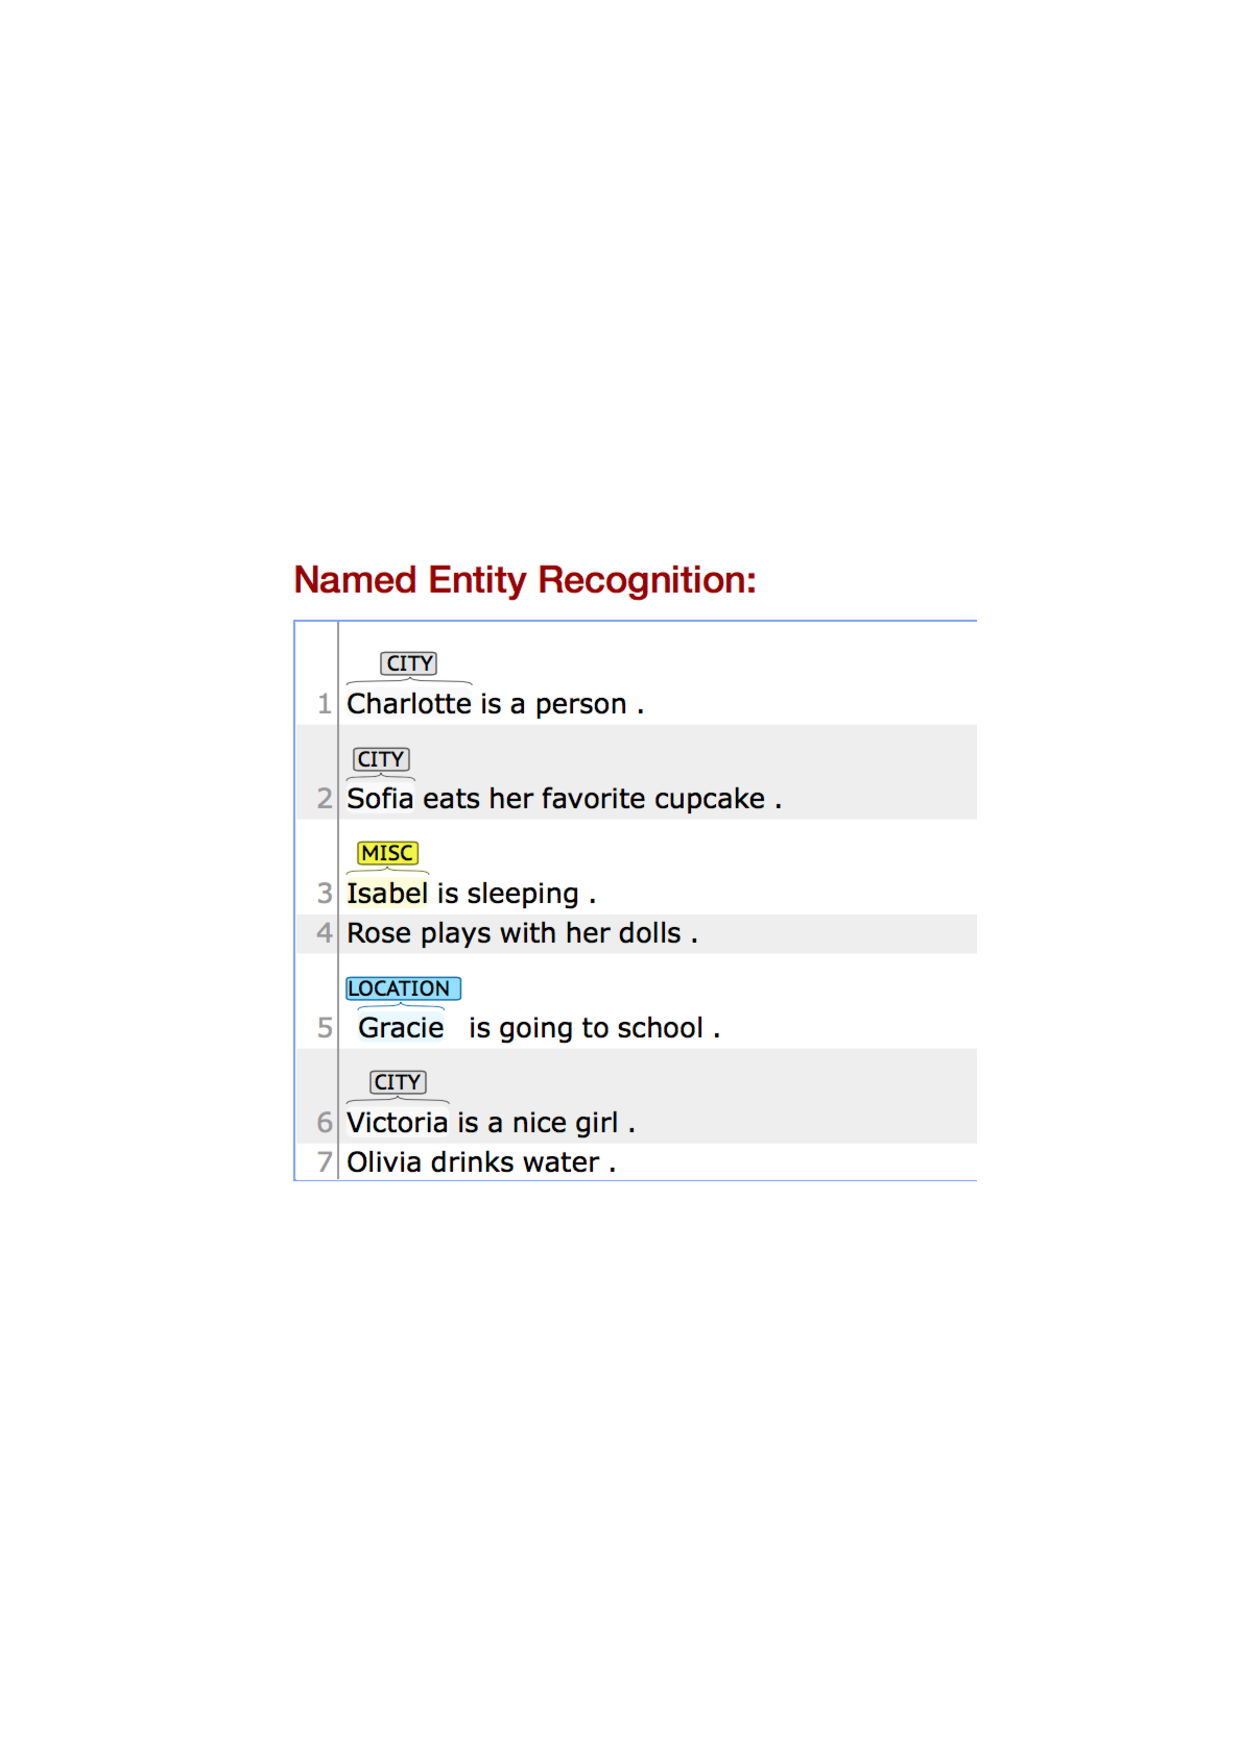
\includegraphics[width=0.45\textwidth,height=0.37\textwidth,trim=0cm 0.25cm 0cm 0cm,clip=true]{motivation.pdf}
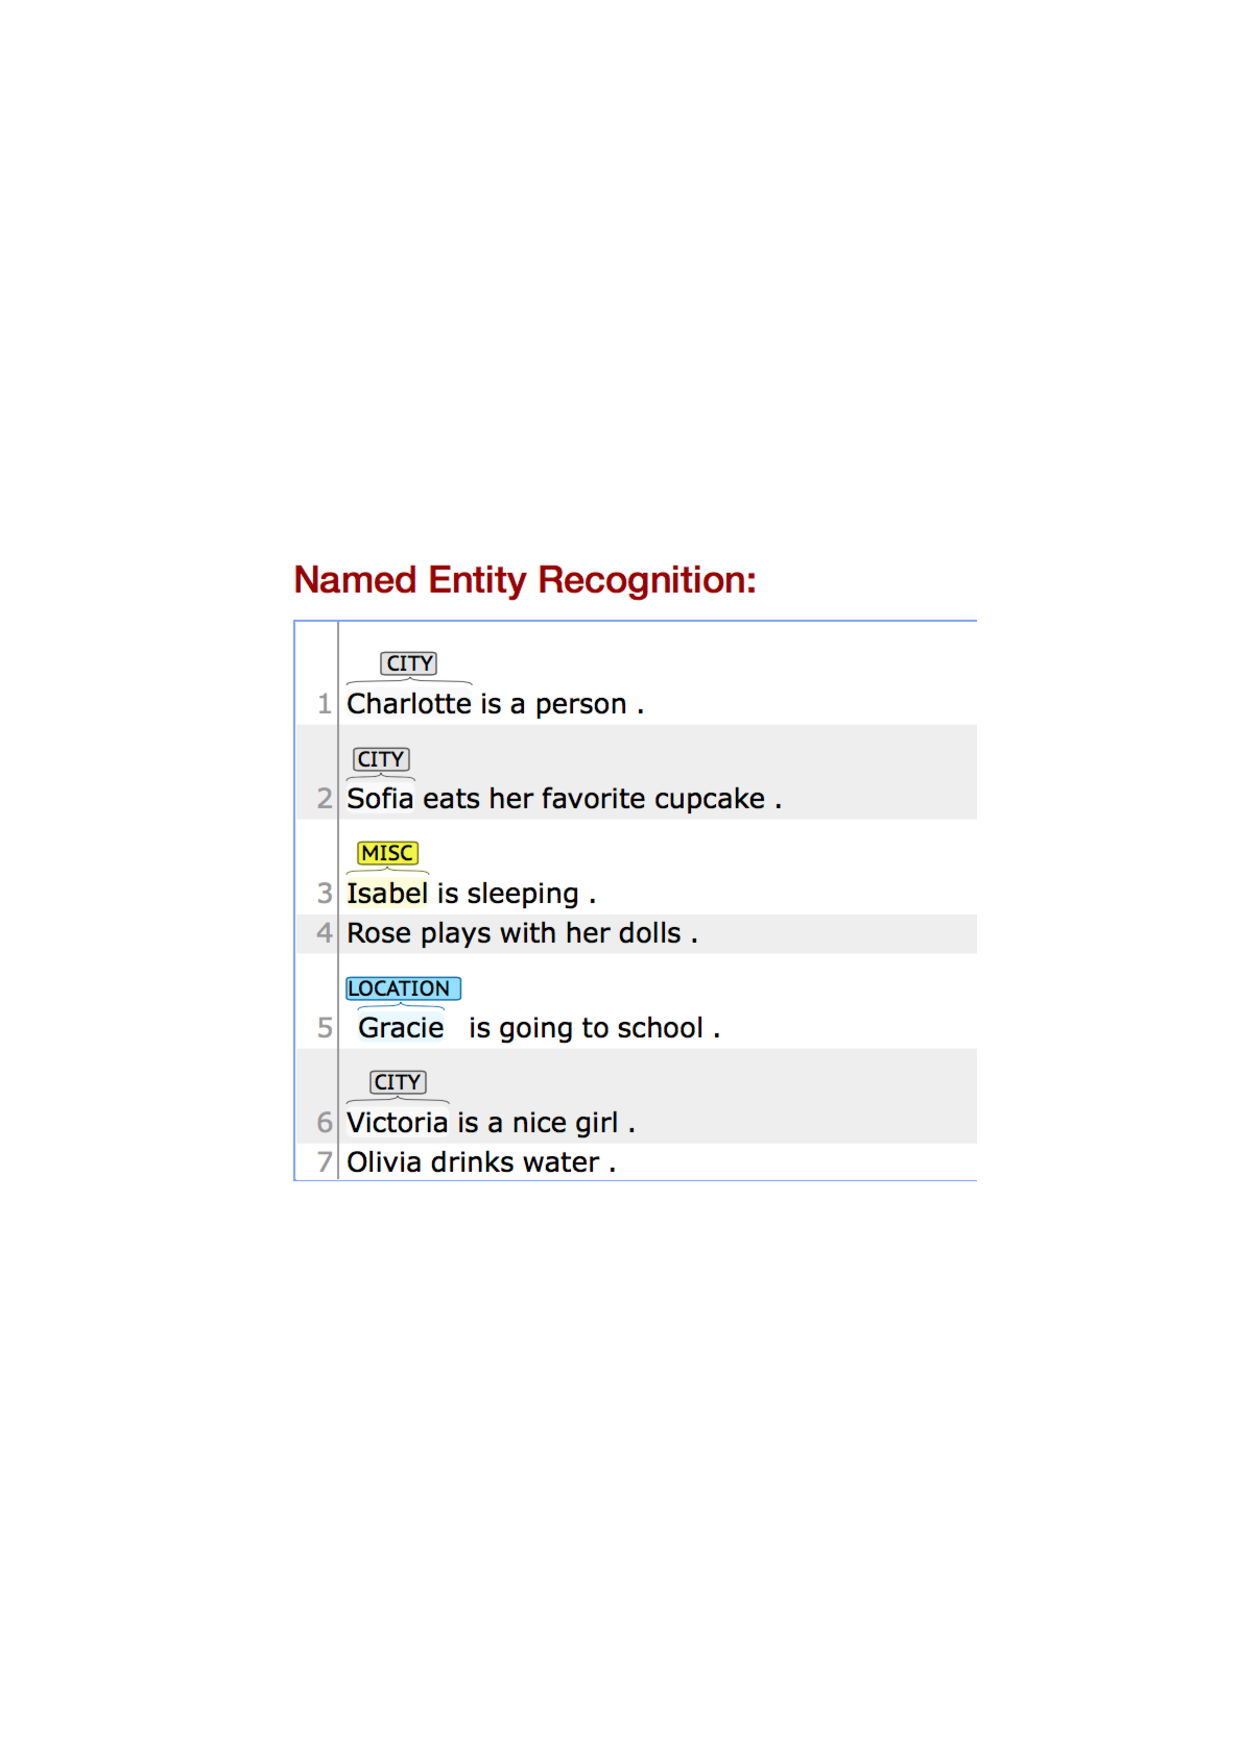
\includegraphics[width=0.45\textwidth,height=0.37\textwidth,trim=4cm 9cm 4cm 9cm,clip=true]{motivation.pdf}
\caption{Examples of PERSON entities that are wrongfully tagged as non-PERSON or NULL entities by CoreNLP.}
\label{motivation}
\end{figure}
We show that there are many instances of such cases throughout history in the real world, and that there are more female names than male names that are incorrectly tagged. Moreover, based on this same U.S. census data, we find that this miscategorization affects more women than men. This serves as our definition of bias which considers the differences between gender groups following the statistical parity notion of fairness \cite{NIPS2017_6995,Dwork:2012:FTA:2090236.2090255}.

The contributions of this paper are fourfold:
\begin{enumerate}
    \item We introduced a benchmark dataset
    %\footnotemark[\ref{projecturl}] 
    that tests NER models for gender bias. This benchmark can be run on any blackbox system.
    \item We studied the existence and extent of gender bias in current NER systems by analysing a 139-year history of names according to the statistical parity notion of fairness \cite{NIPS2017_6995,Dwork:2012:FTA:2090236.2090255}.
    \item We compared different versions of models and found that newer versions are amplifying gender bias in an effort to boost performance. Based on our observations, we defined a new source of bias that arises from version updates in the systems. 
    \item Finally, we analyzed datasets currently used for training many NER models and found the extent of gender bias in these datasets.
\end{enumerate}
% \begin{figure*}[!bt]
% \begin{subfigure}[t]{\textwidth}
% 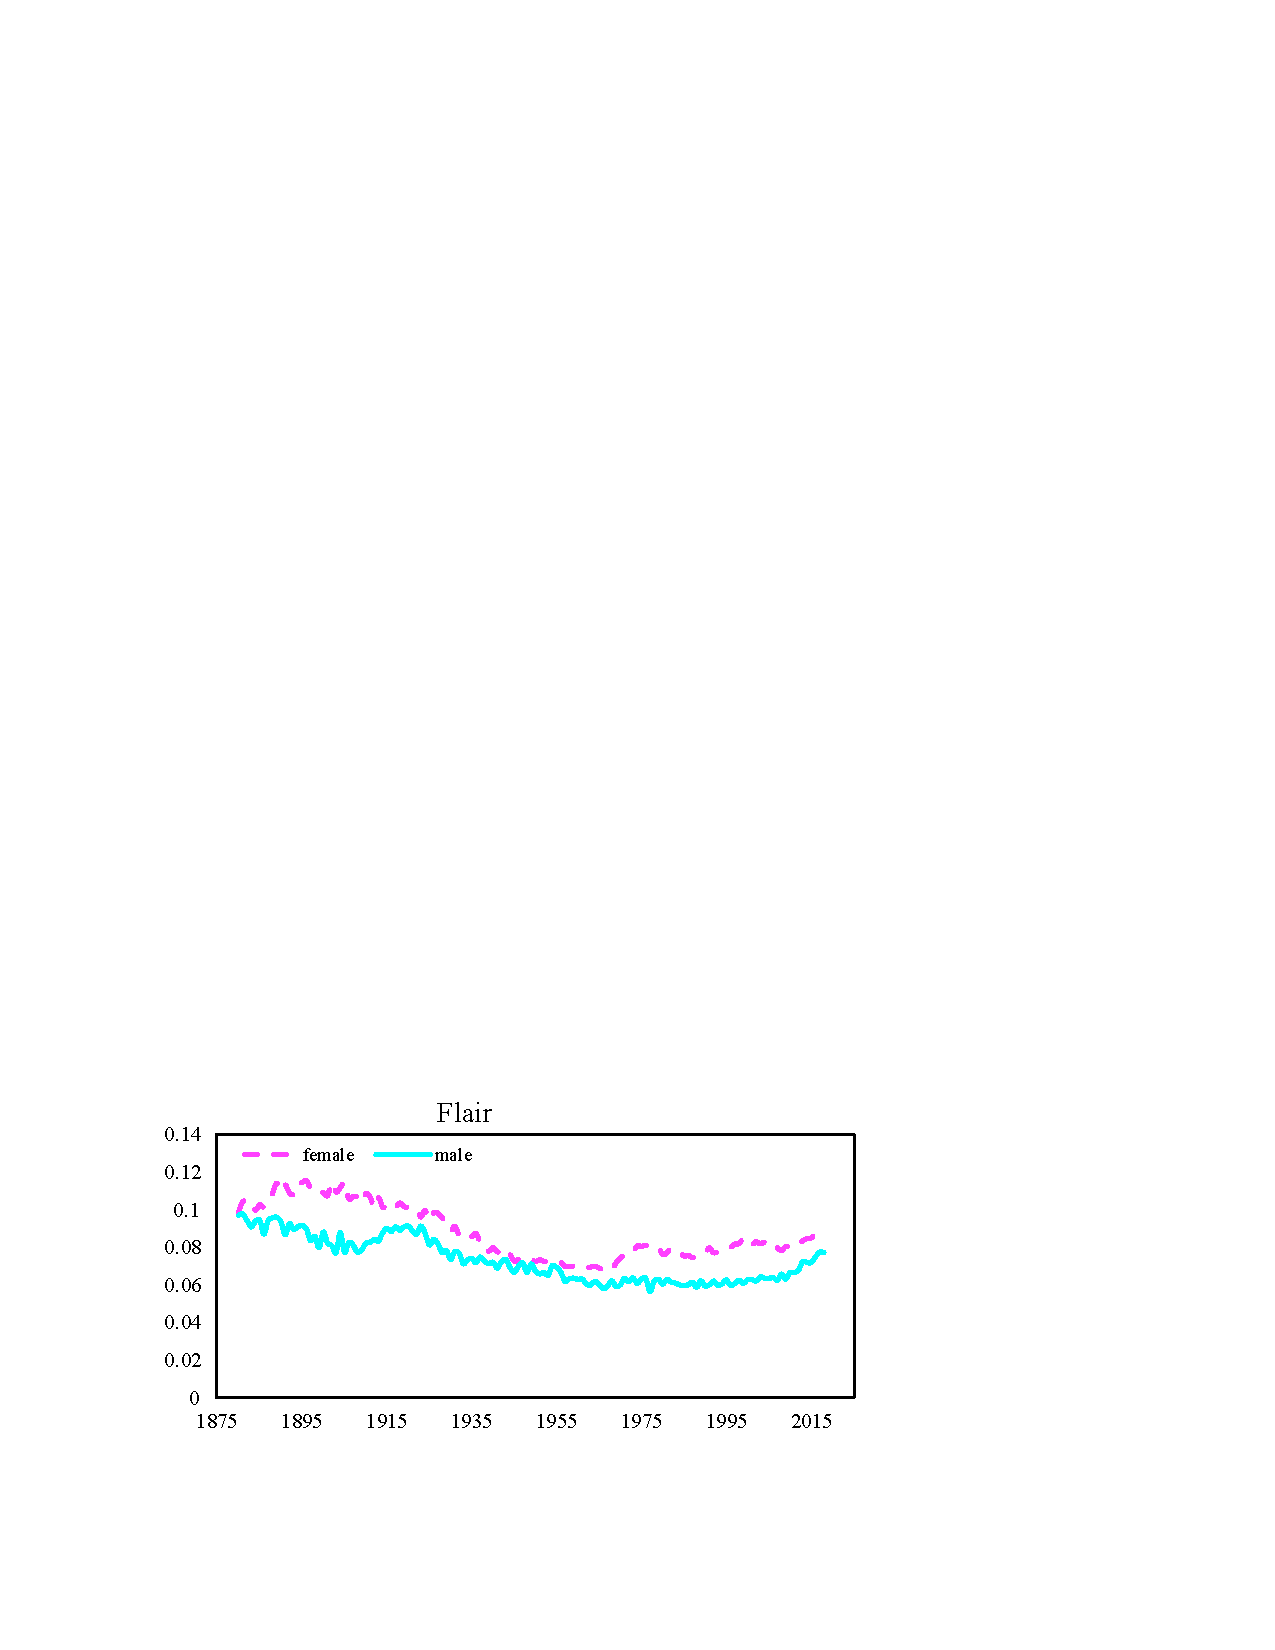
\includegraphics[width=0.196\textwidth,height=0.15\textwidth,trim=0cm 0cm 0cm 0cm,clip=true]{images/unweighted_type1/unweighted_type1_1.pdf}
% 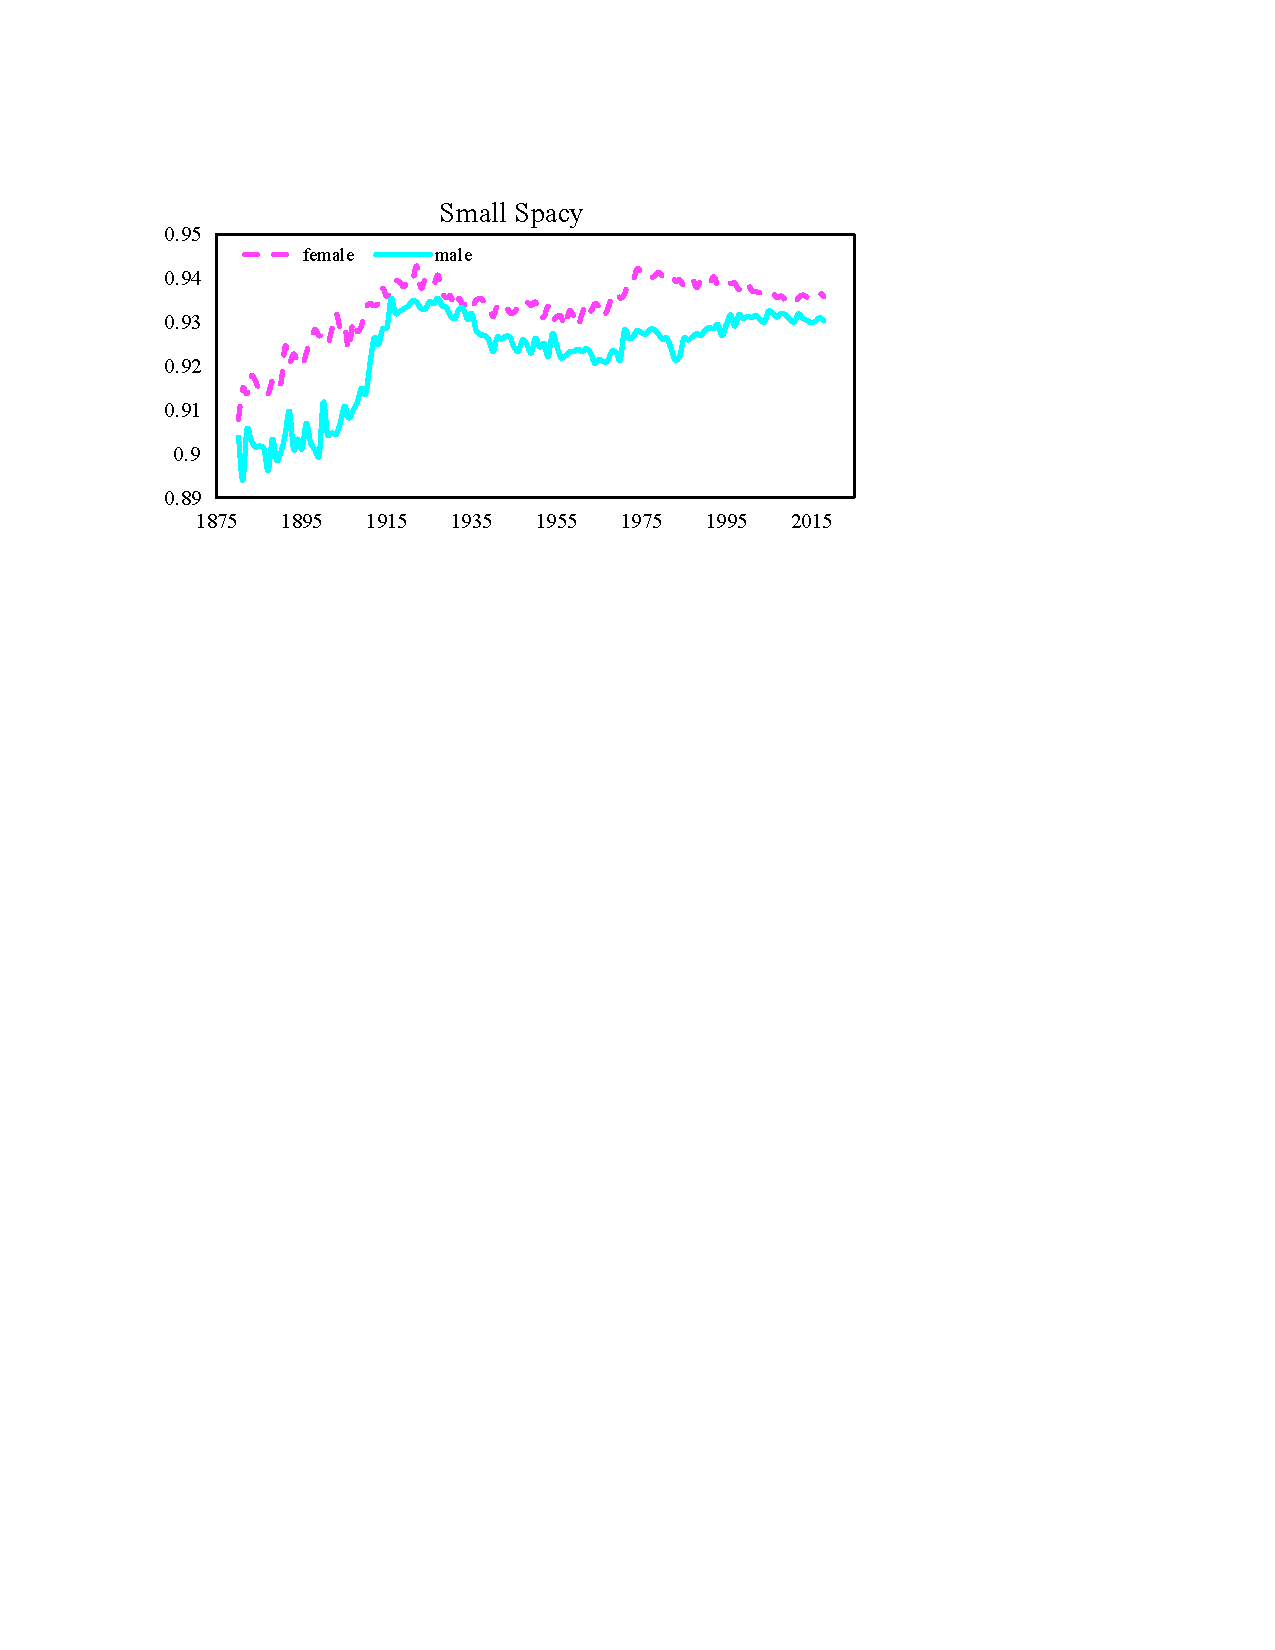
\includegraphics[width=0.196\textwidth,height=0.15\textwidth,trim=0cm 0cm 0cm 0cm,clip=true]{images/unweighted_type1/unweighted_type1_2.pdf}
% 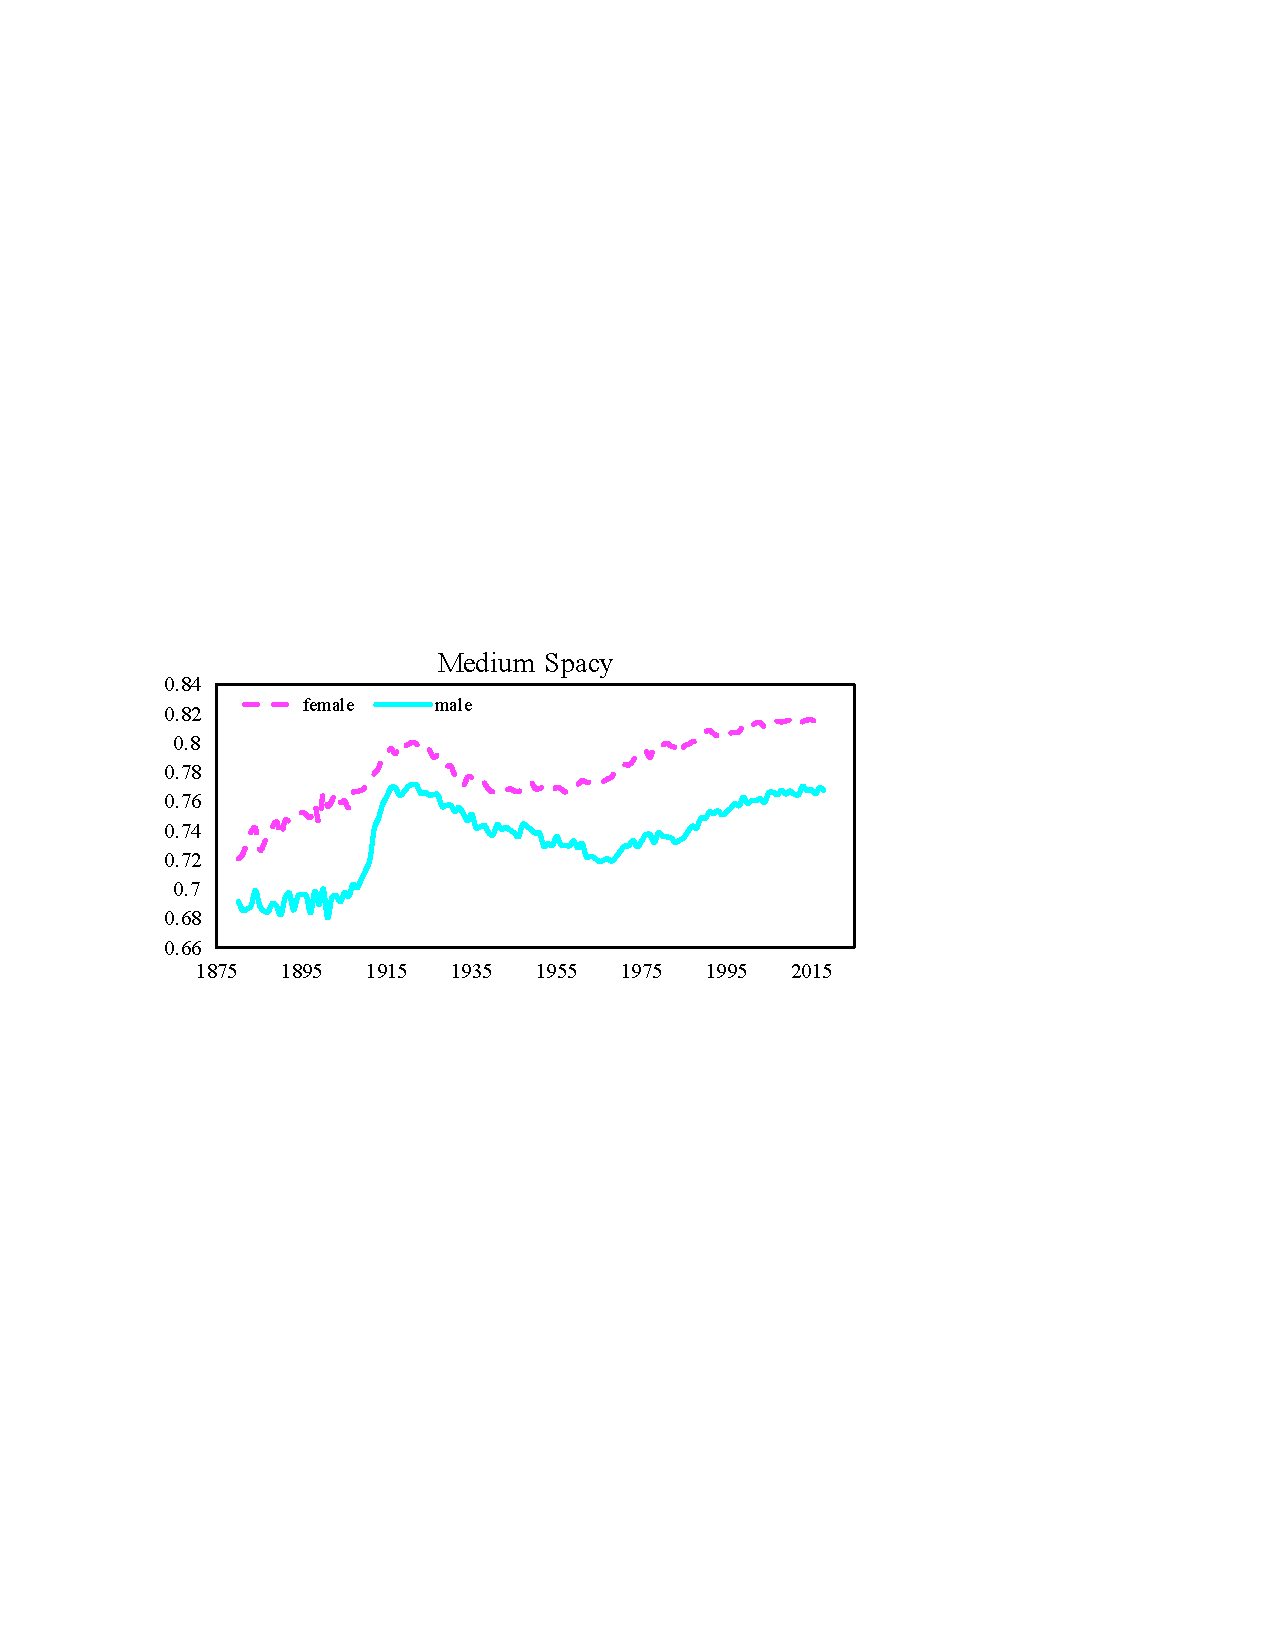
\includegraphics[width=0.196\textwidth,height=0.15\textwidth,trim=0cm 0cm 0cm 0cm,clip=true]{images/unweighted_type1/unweighted_type1_3.pdf}
% 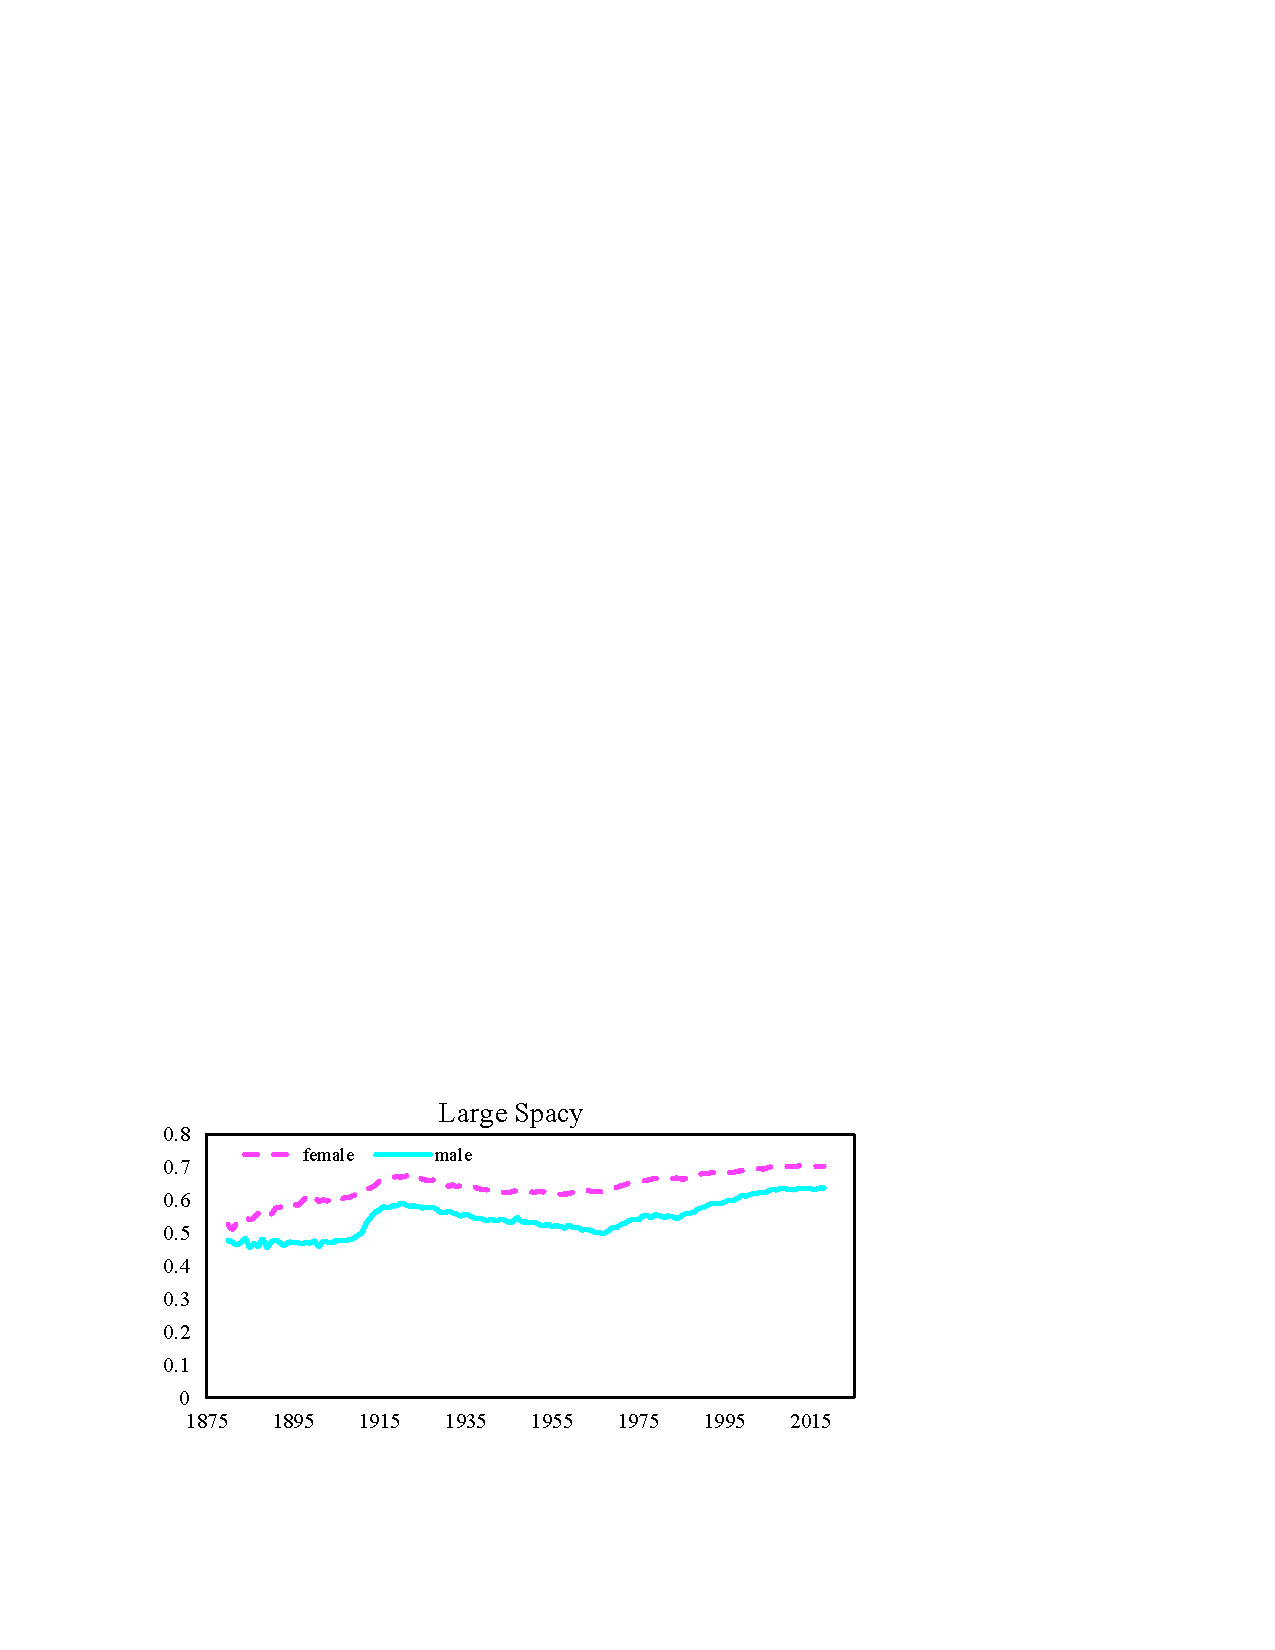
\includegraphics[width=0.196\textwidth,height=0.15\textwidth,trim=0cm 0cm 0cm 0cm,clip=true]{images/unweighted_type1/unweighted_type1_4.pdf}
% 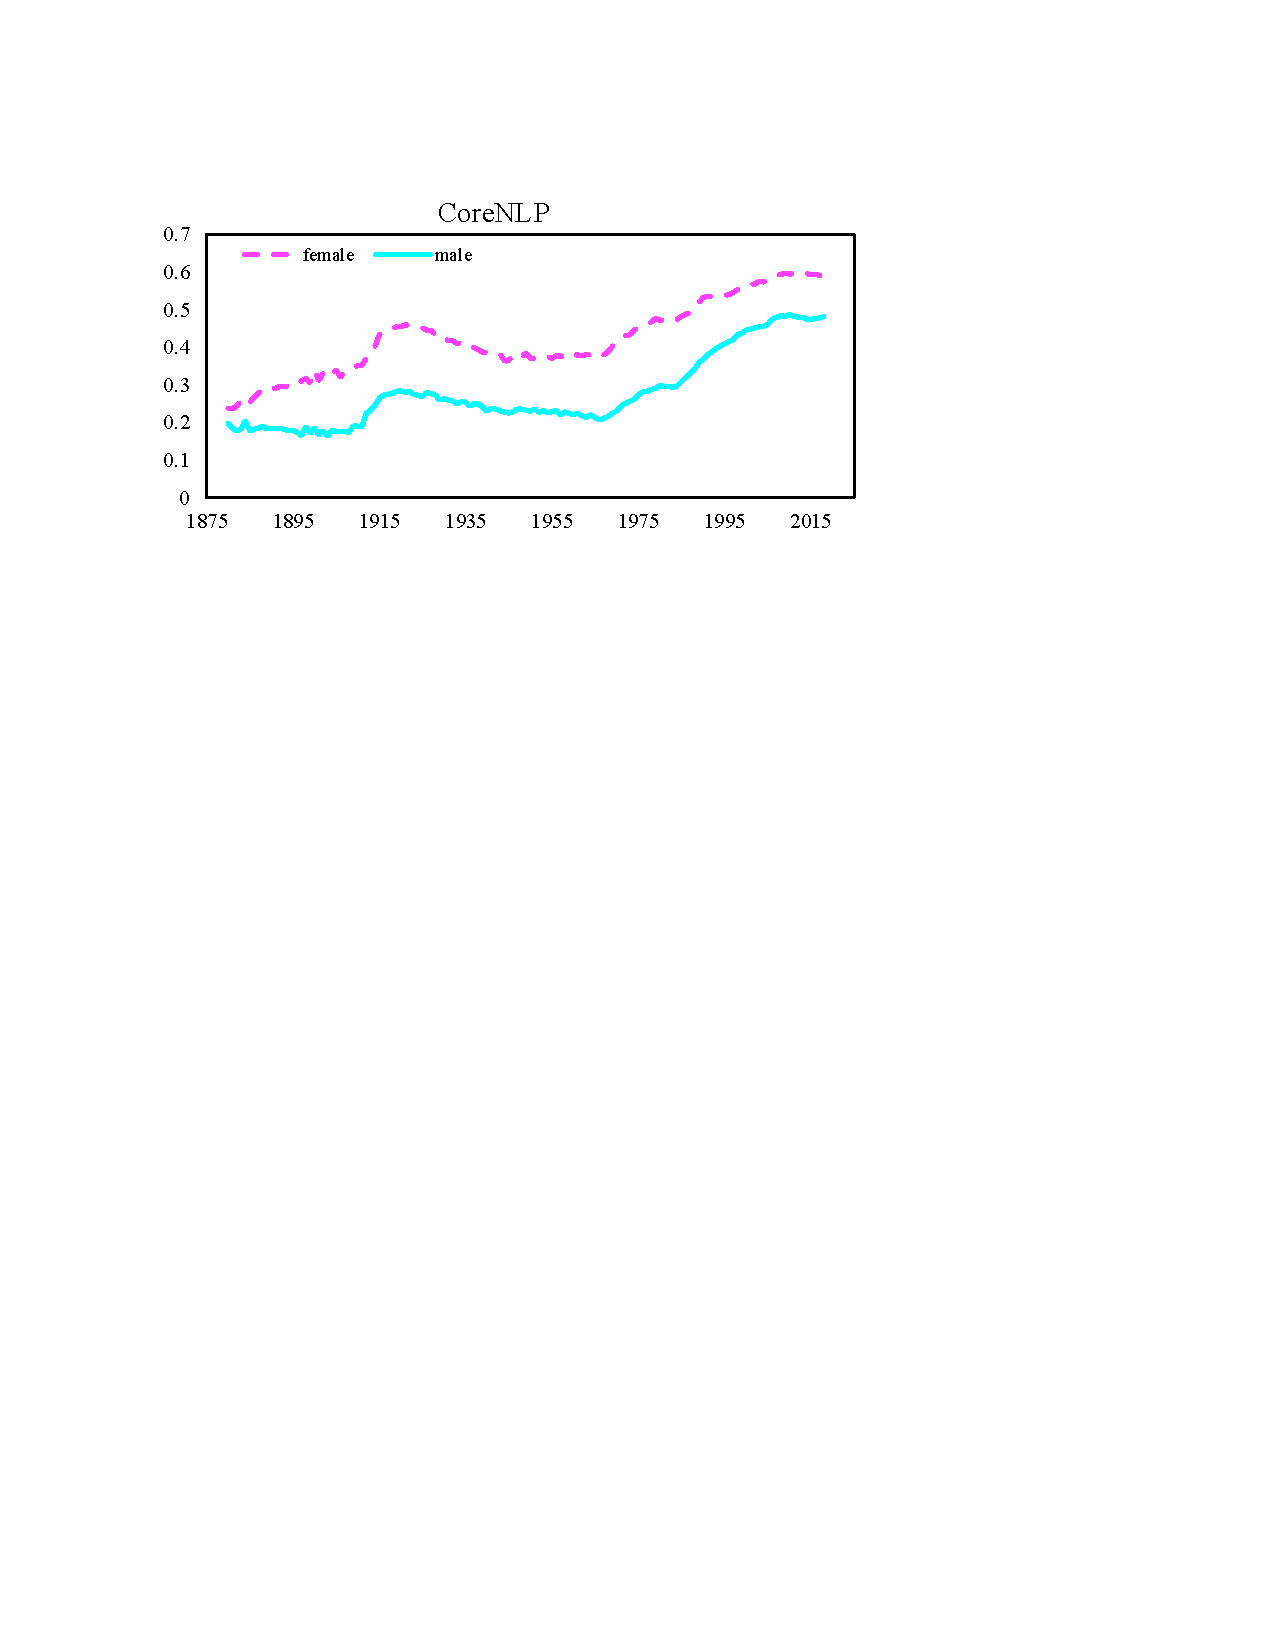
\includegraphics[width=0.196\textwidth,height=0.15\textwidth,trim=0cm 0cm 0cm 0cm,clip=true]{images/unweighted_type1/unweighted_type1_5.pdf}
% \caption{Error Type-1 Unweighted}
% \end{subfigure}
% \begin{subfigure}[t]{\textwidth}
% 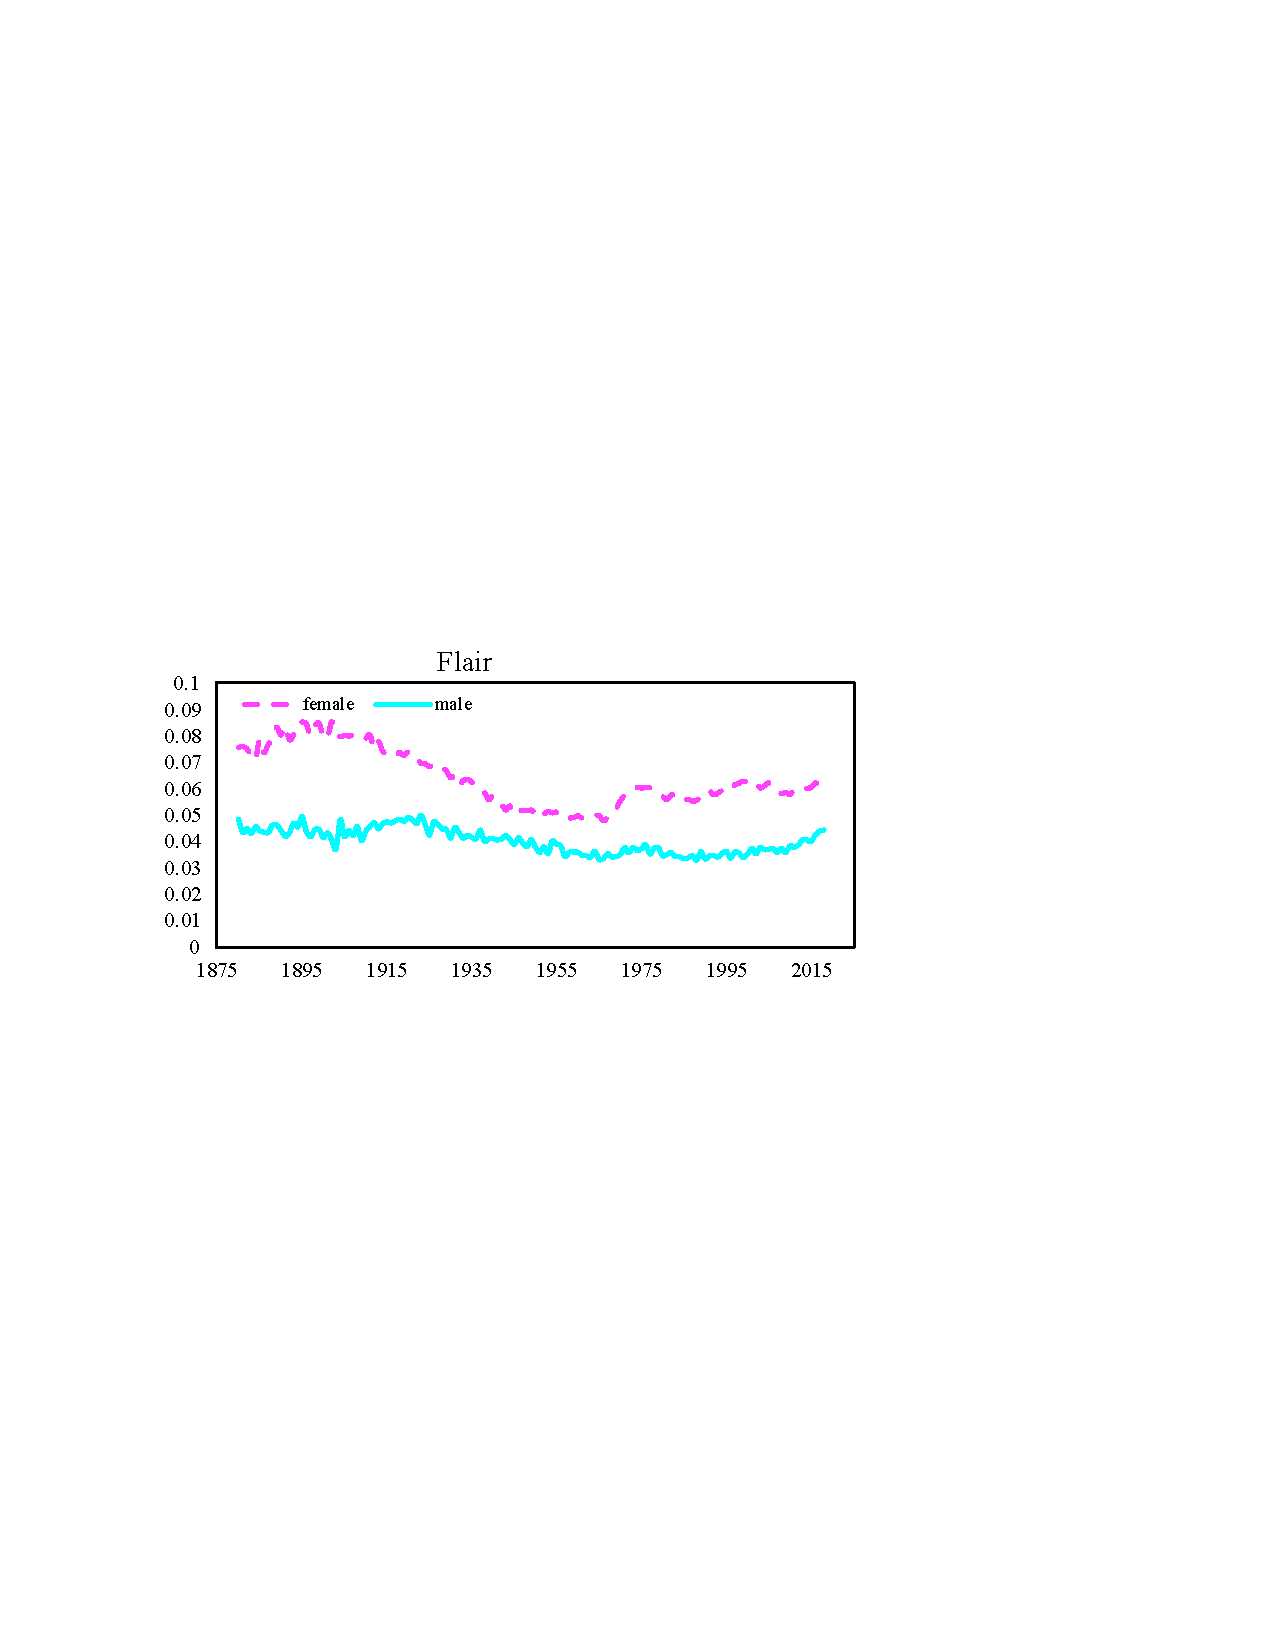
\includegraphics[width=0.196\textwidth,height=0.15\textwidth,trim=0cm 0cm 0cm 0cm,clip=true]{images/unweighted_type2/unweighted_type2_1.pdf}
% 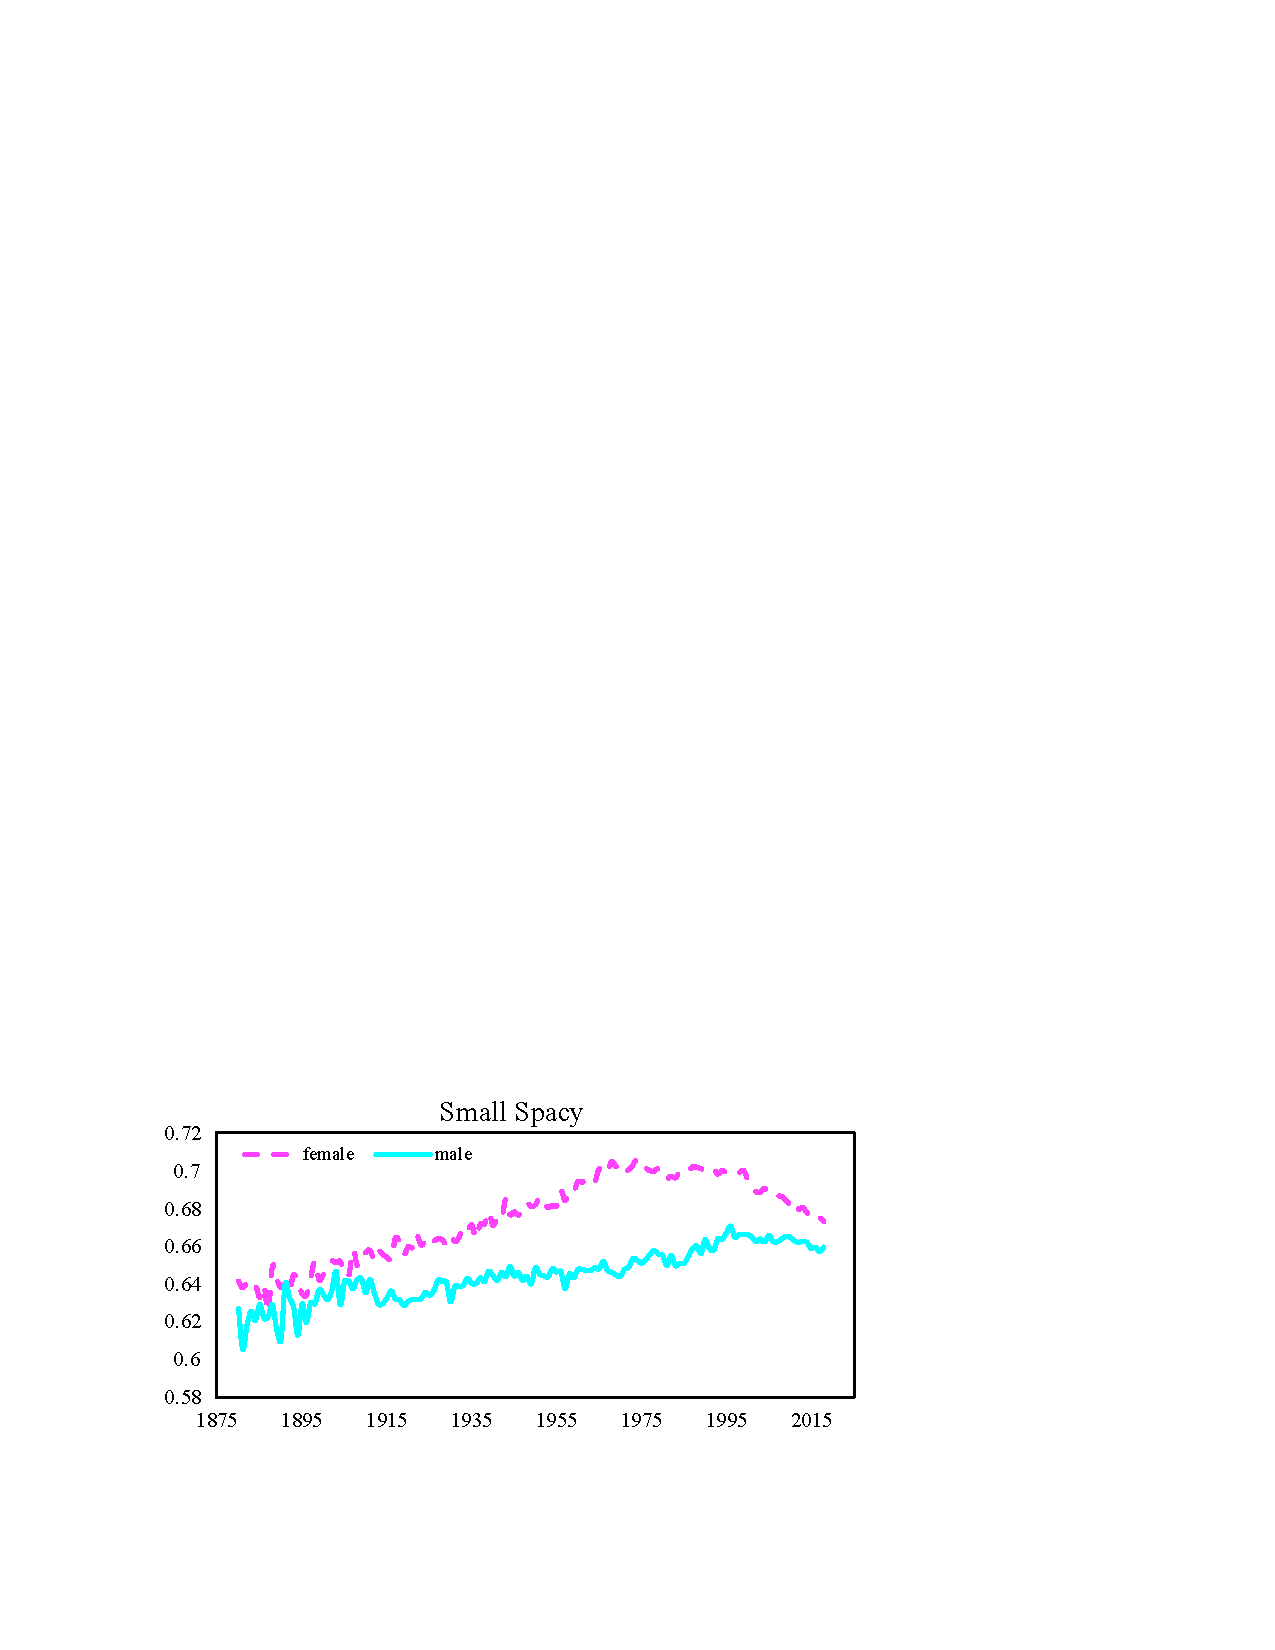
\includegraphics[width=0.196\textwidth,height=0.15\textwidth,trim=0cm 0cm 0cm 0cm,clip=true]{images/unweighted_type2/unweighted_type2_2.pdf}
% 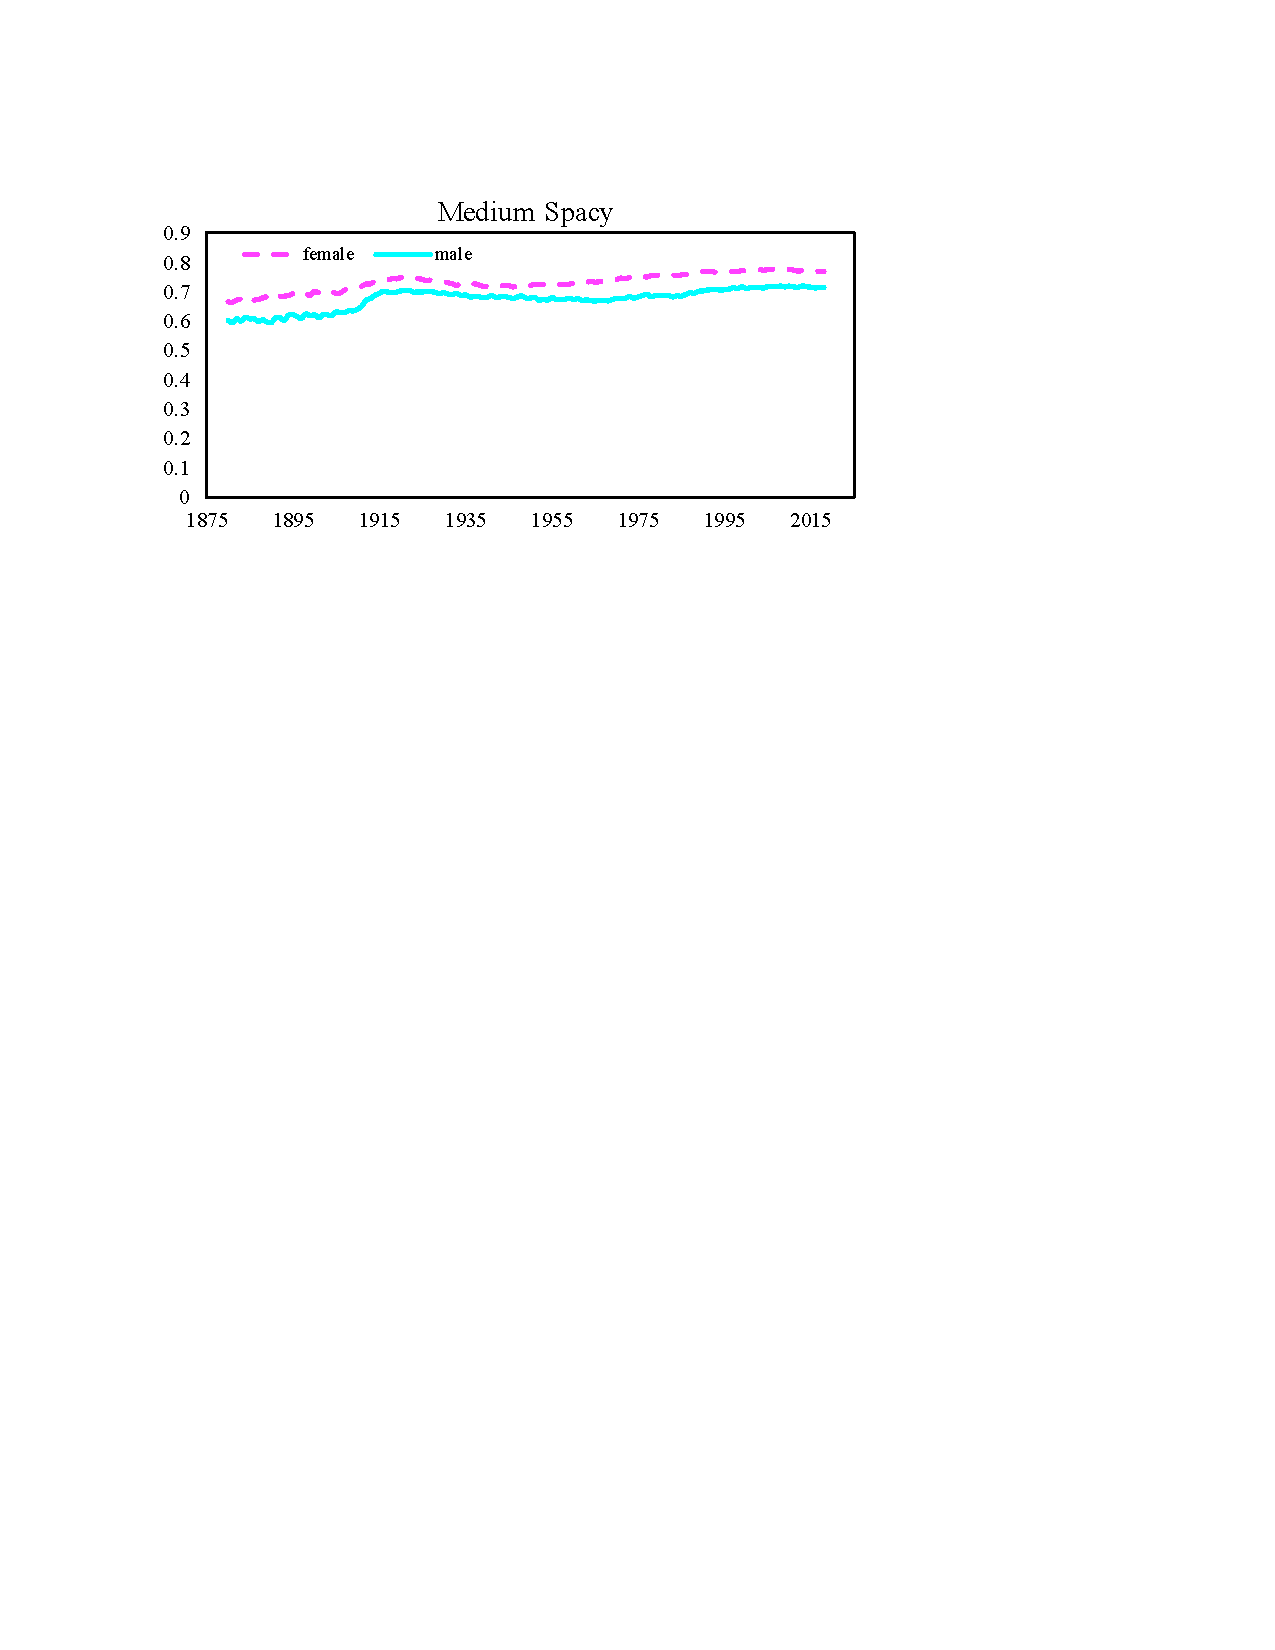
\includegraphics[width=0.196\textwidth,height=0.15\textwidth,trim=0cm 0cm 0cm 0cm,clip=true]{images/unweighted_type2/unweighted_type2_3.pdf}
% 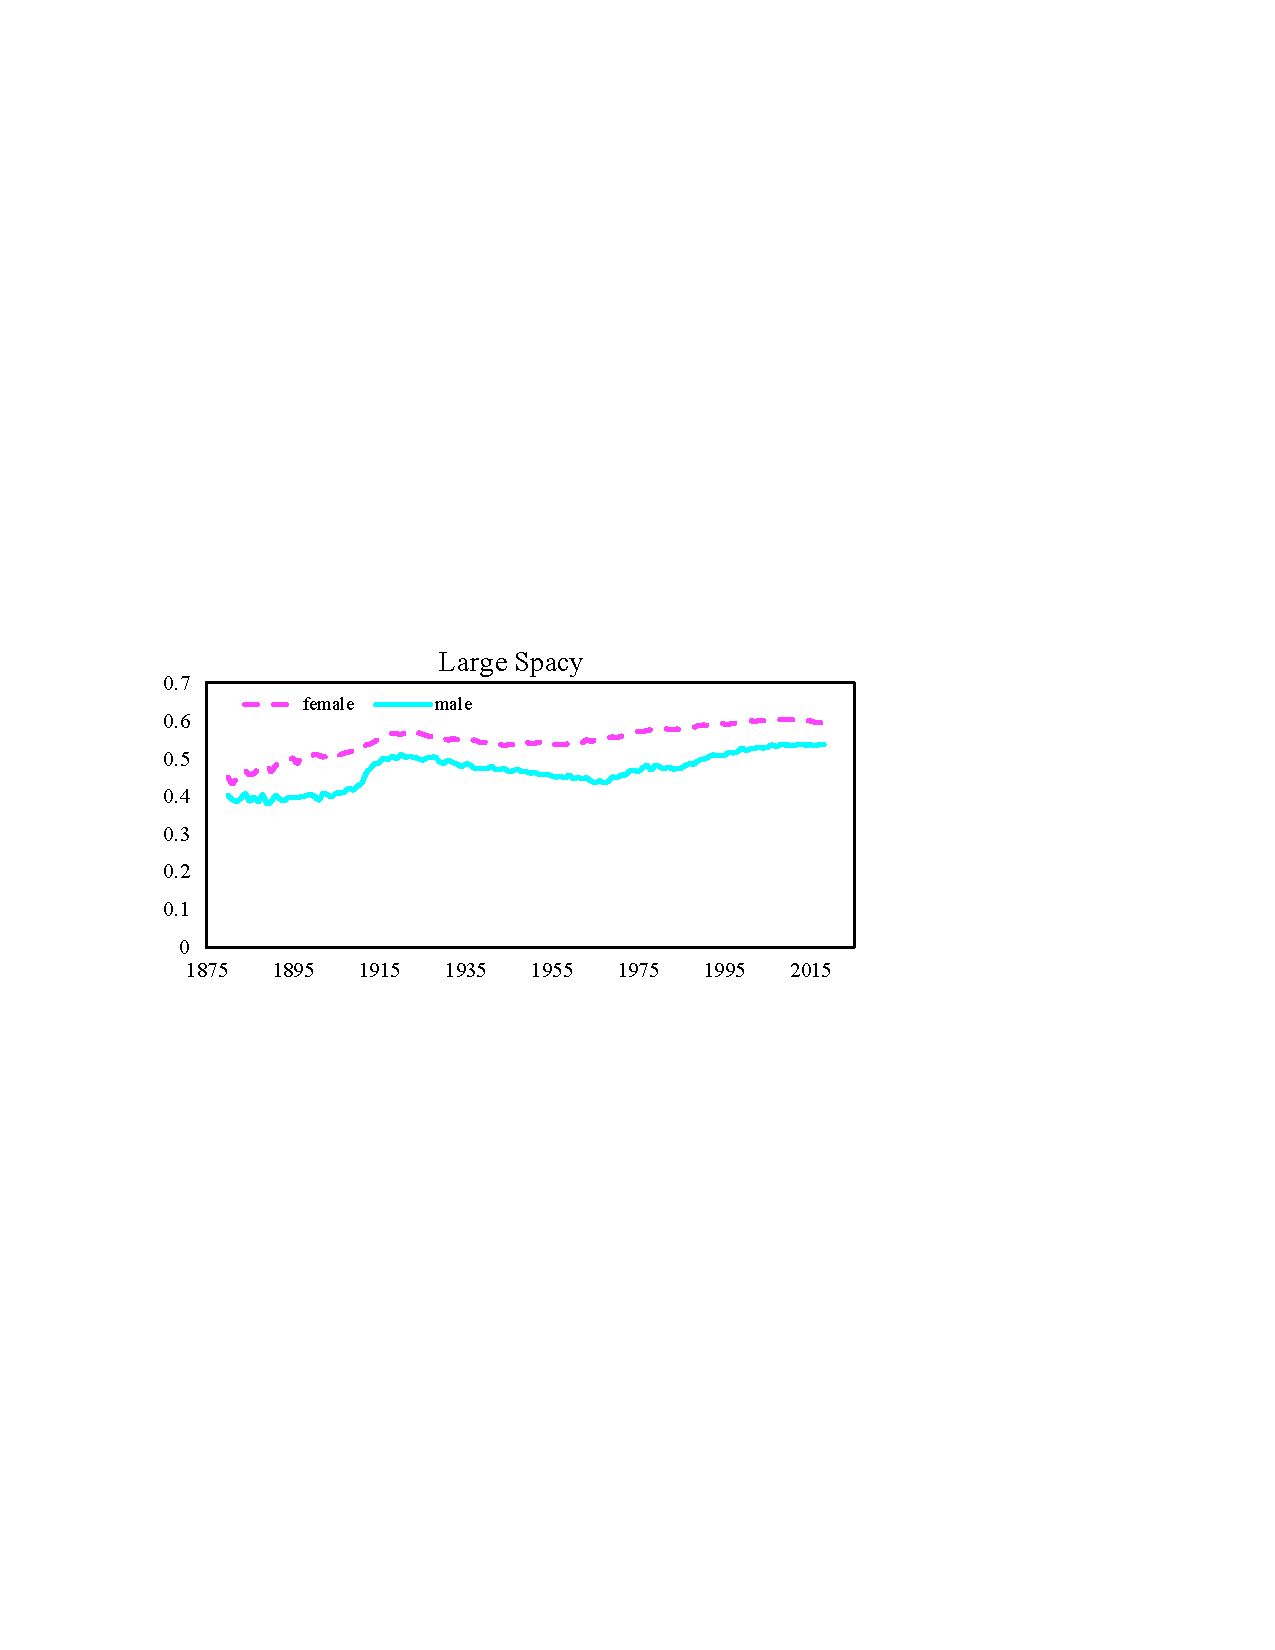
\includegraphics[width=0.196\textwidth,height=0.15\textwidth,trim=0cm 0cm 0cm 0cm,clip=true]{images/unweighted_type2/unweighted_type2_4.pdf}
% 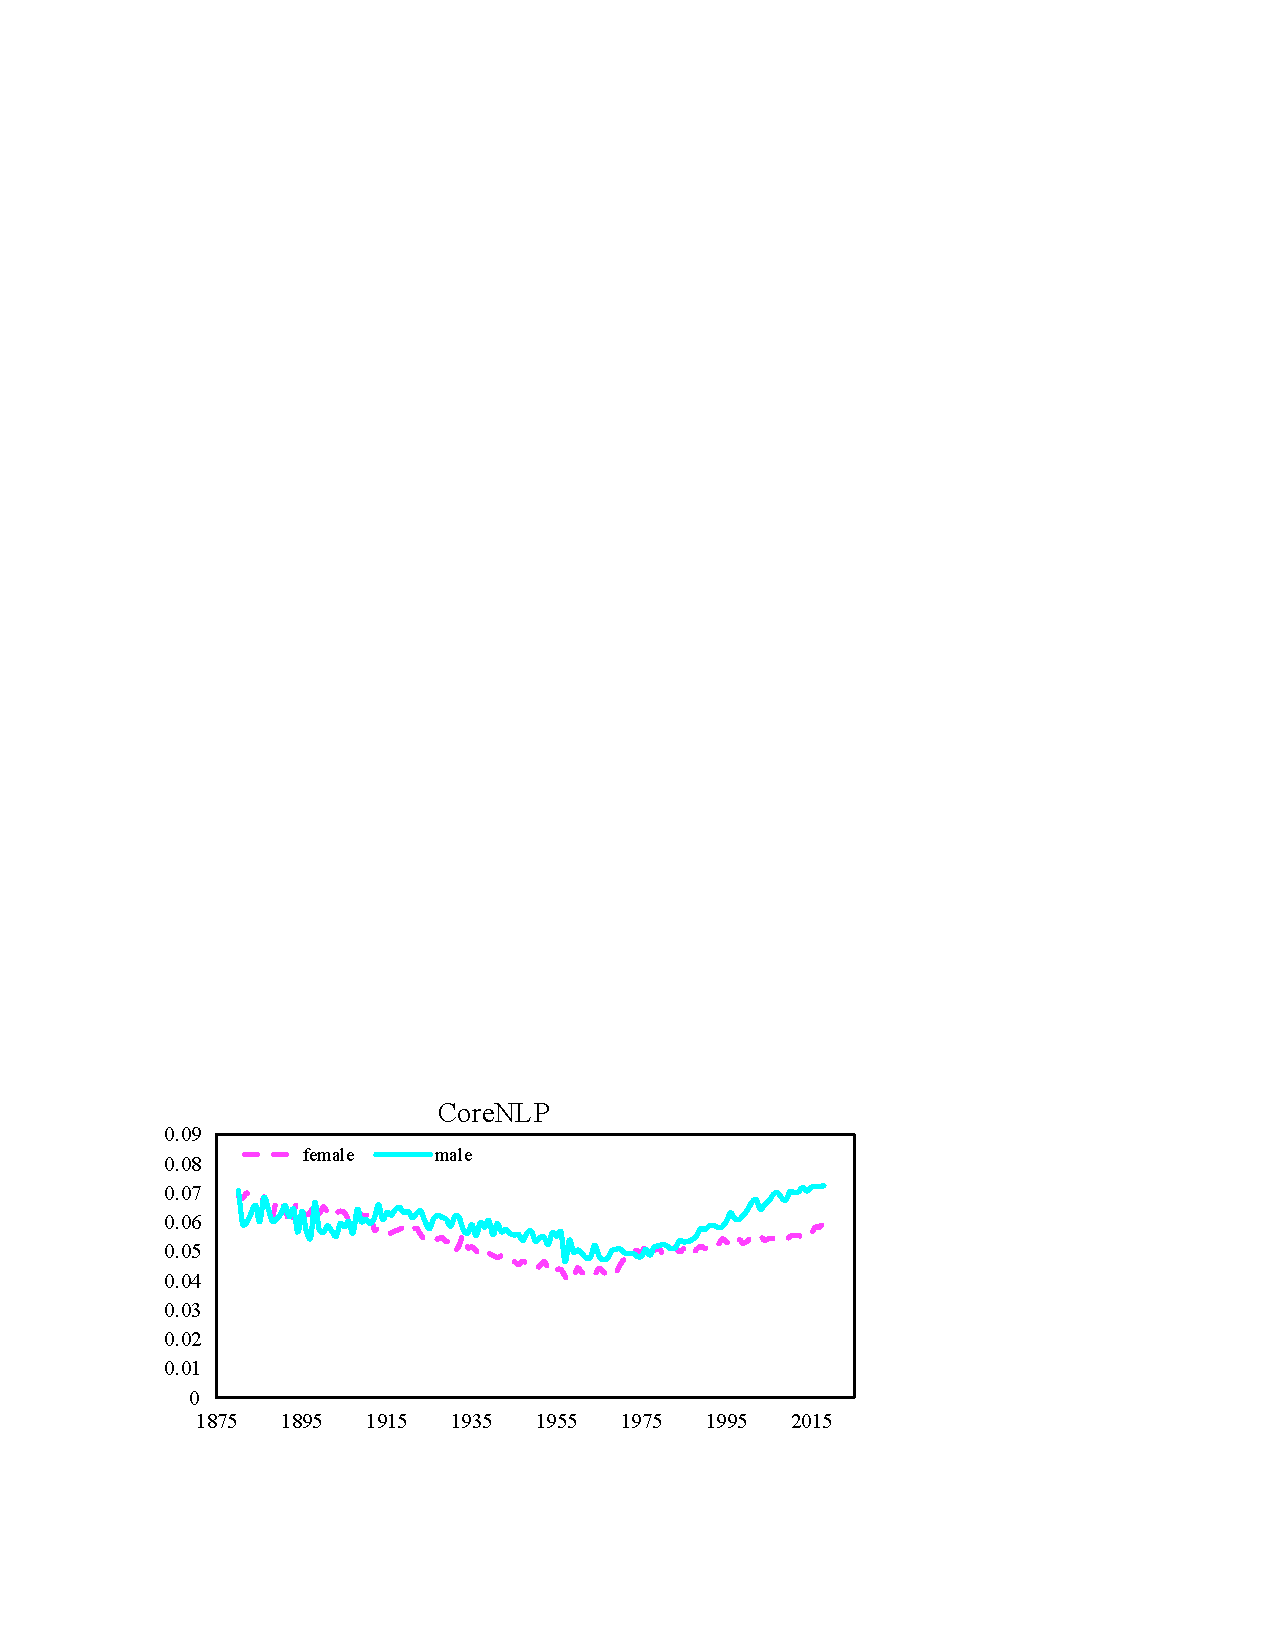
\includegraphics[width=0.196\textwidth,height=0.15\textwidth,trim=0cm 0cm 0cm 0cm,clip=true]{images/unweighted_type2/unweighted_type2_5.pdf}
% \caption{Error Type-2 Unweighted}
% \end{subfigure}
% \begin{subfigure}[t]{\textwidth}
% 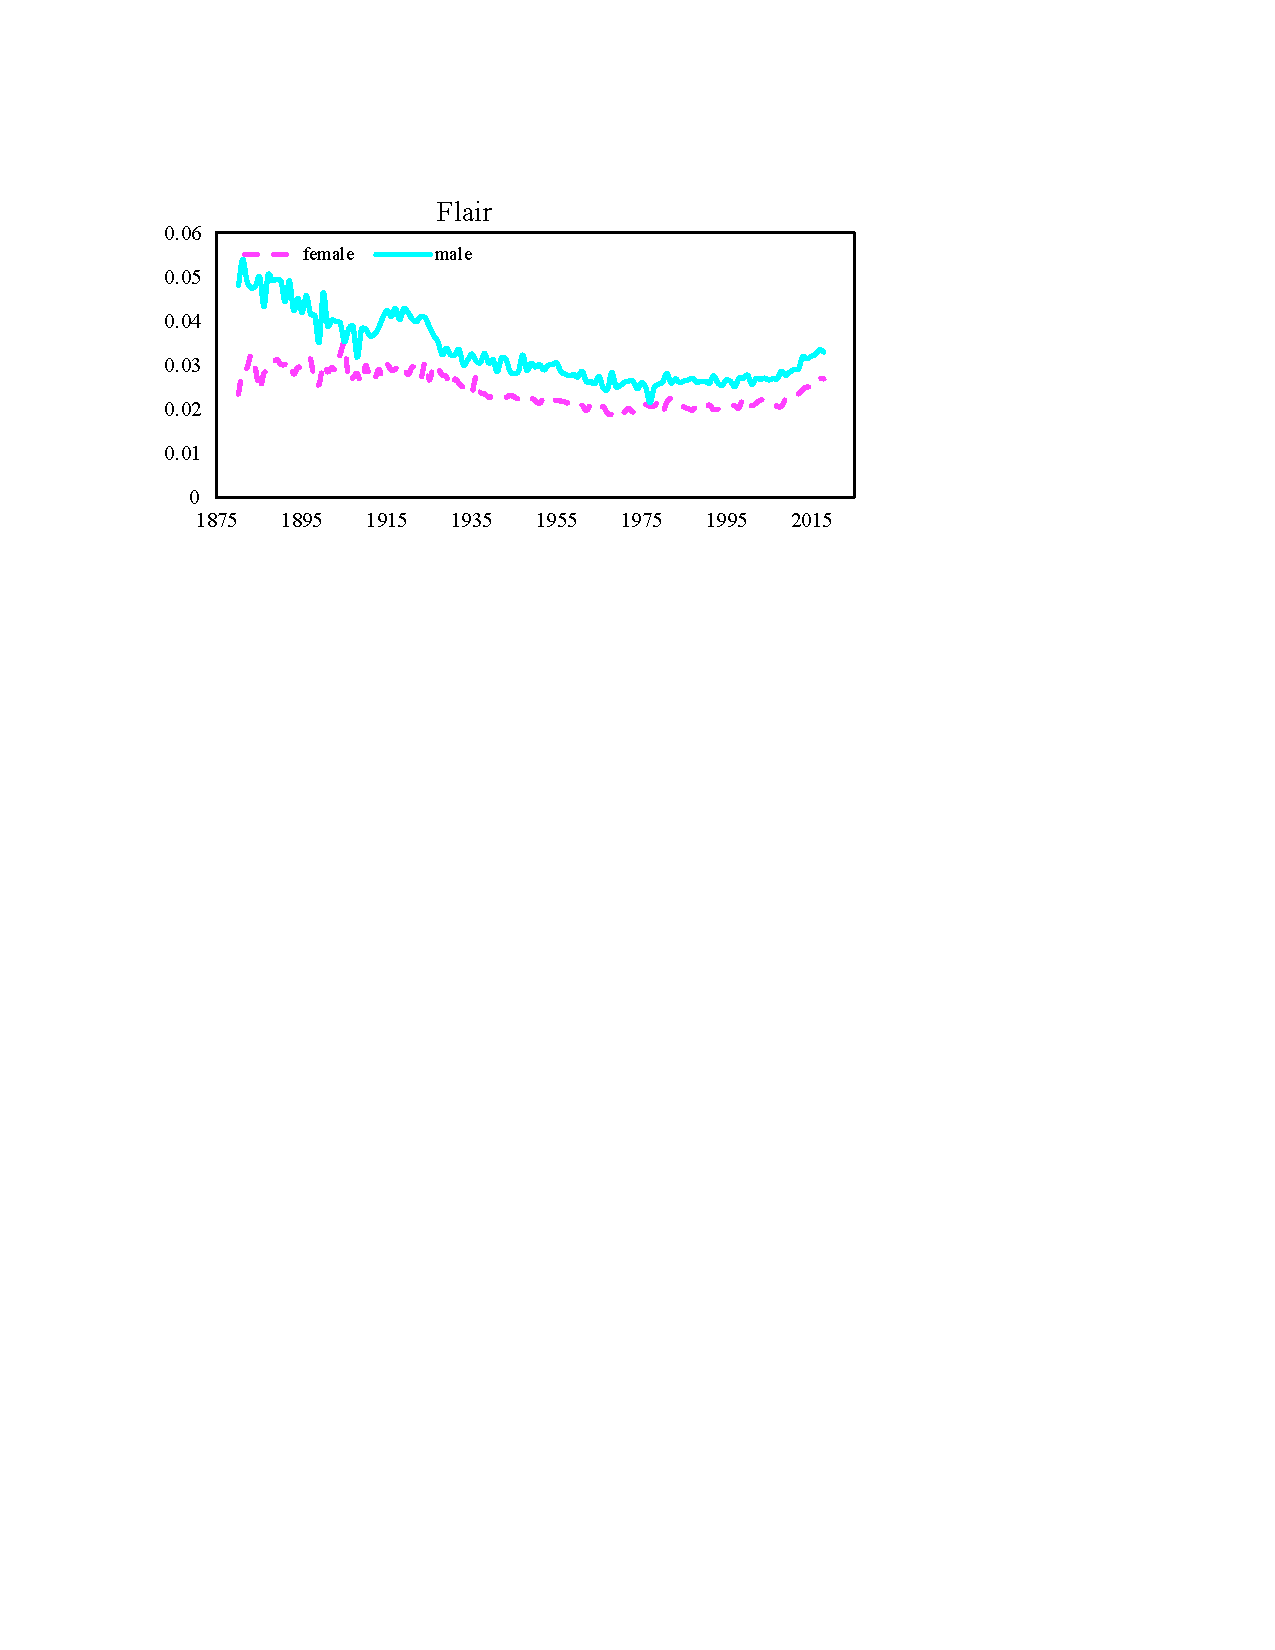
\includegraphics[width=0.196\textwidth,height=0.15\textwidth,trim=0cm 0cm 0cm 0cm,clip=true]{images/unweighted_type3/unweighted_type3_1.pdf}
% 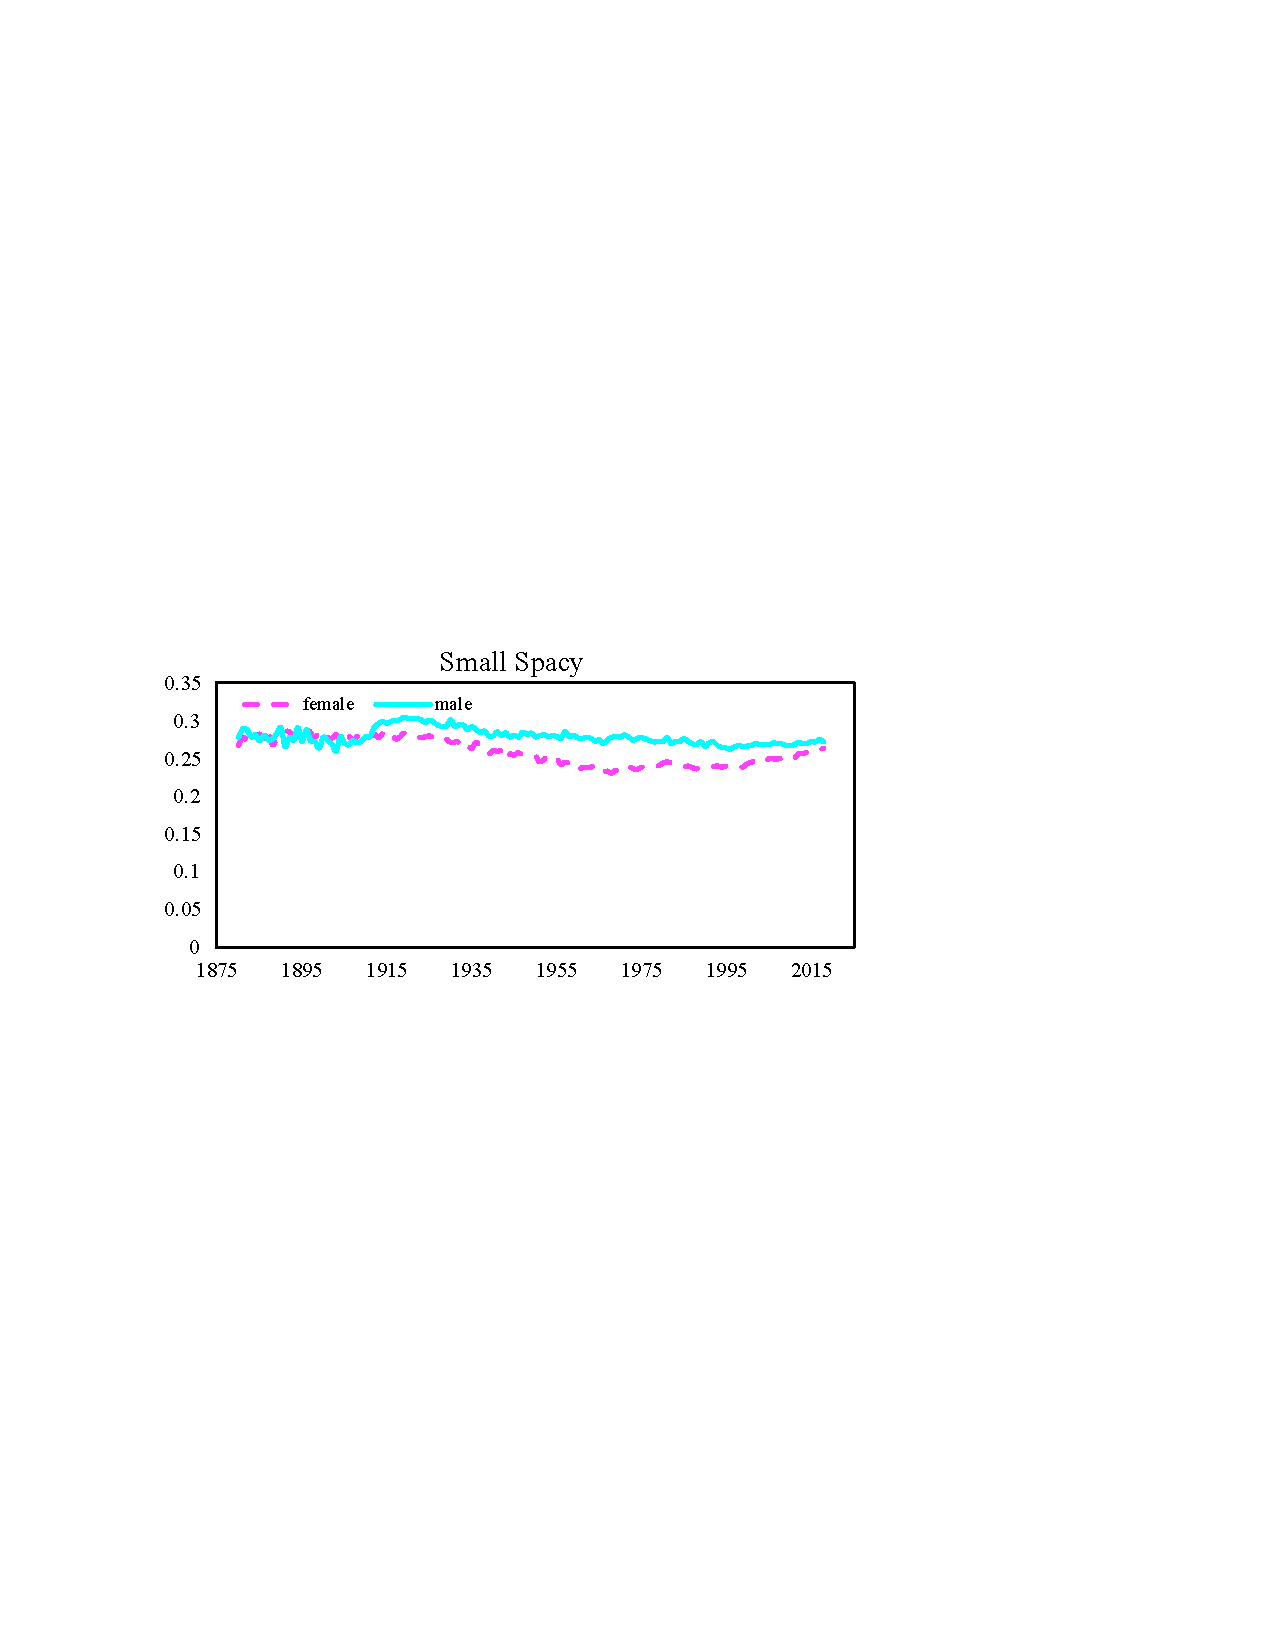
\includegraphics[width=0.196\textwidth,height=0.15\textwidth,trim=0cm 0cm 0cm 0cm,clip=true]{images/unweighted_type3/unweighted_type3_2.pdf}
% 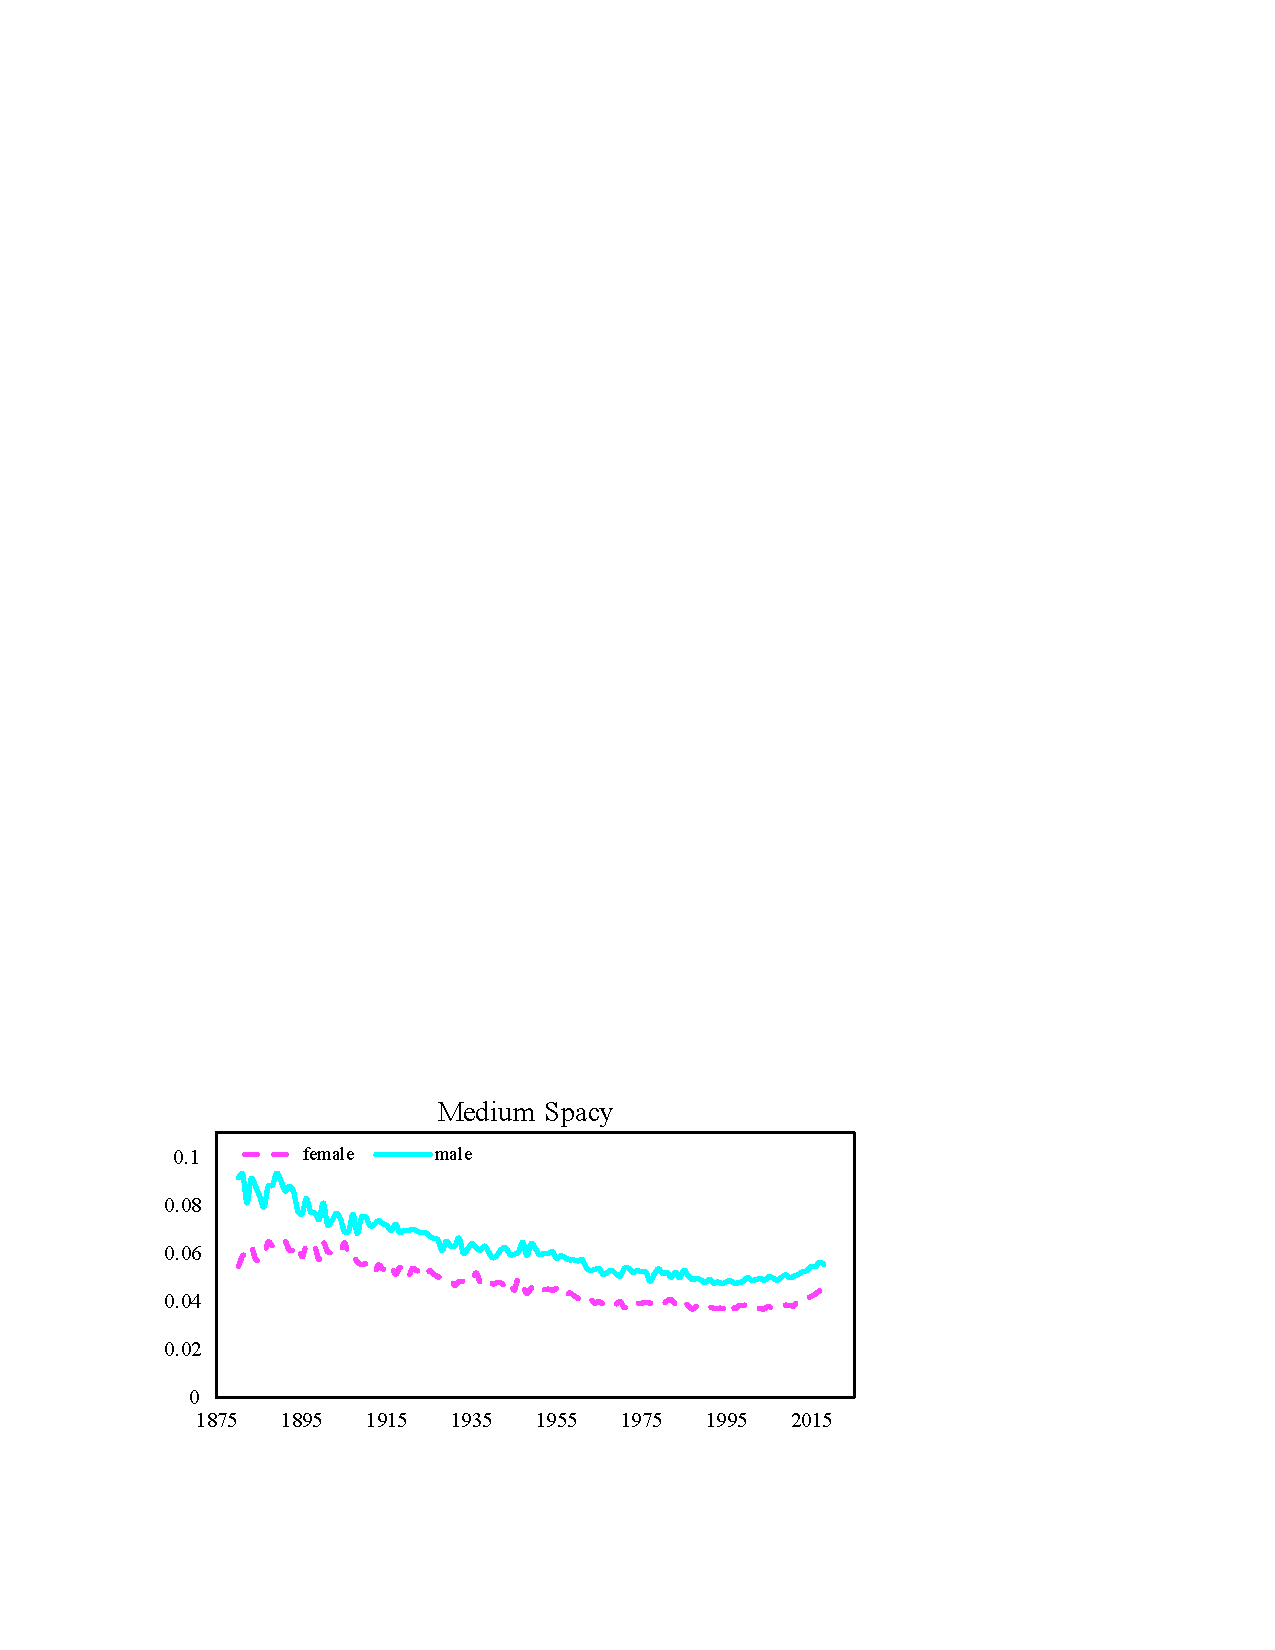
\includegraphics[width=0.196\textwidth,height=0.15\textwidth,trim=0cm 0cm 0cm 0cm,clip=true]{images/unweighted_type3/unweighted_type3_3.pdf}
% 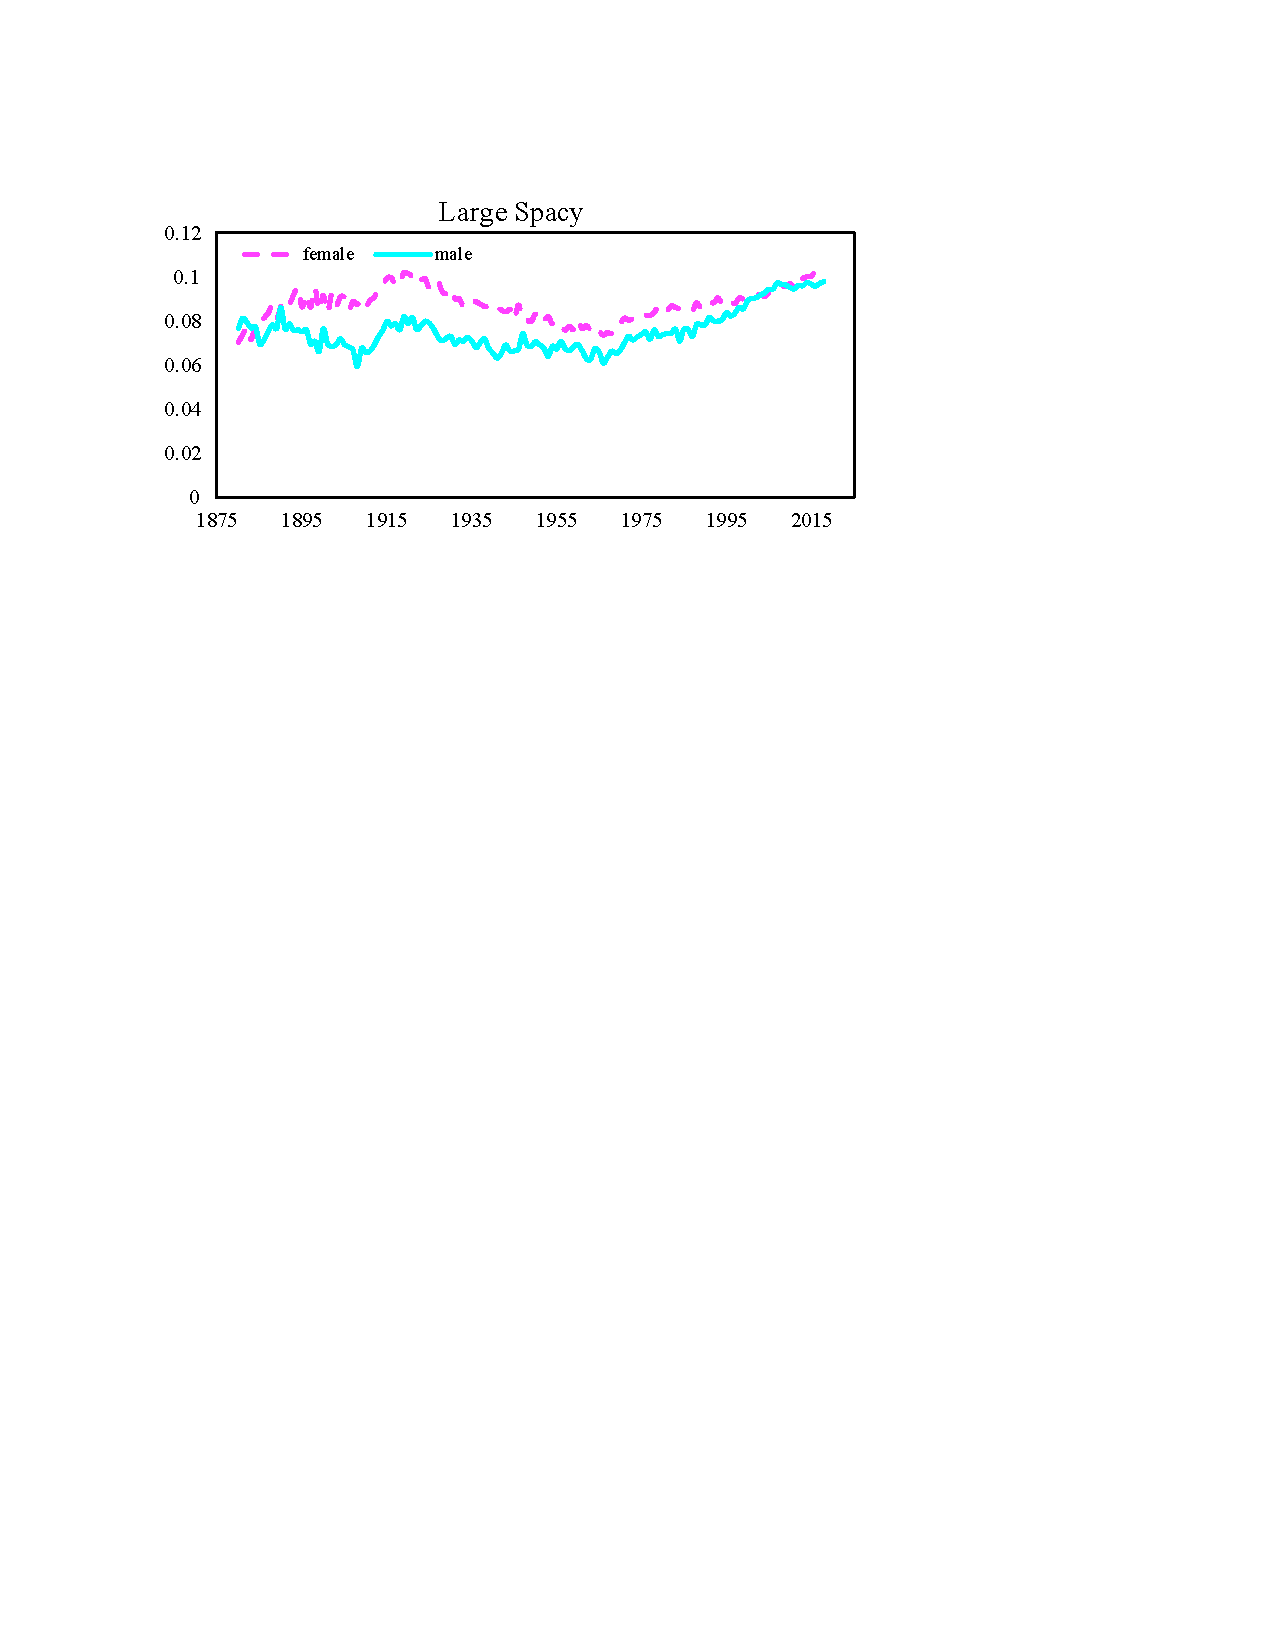
\includegraphics[width=0.196\textwidth,height=0.15\textwidth,trim=0cm 0cm 0cm 0cm,clip=true]{images/unweighted_type3/unweighted_type3_4.pdf}
% 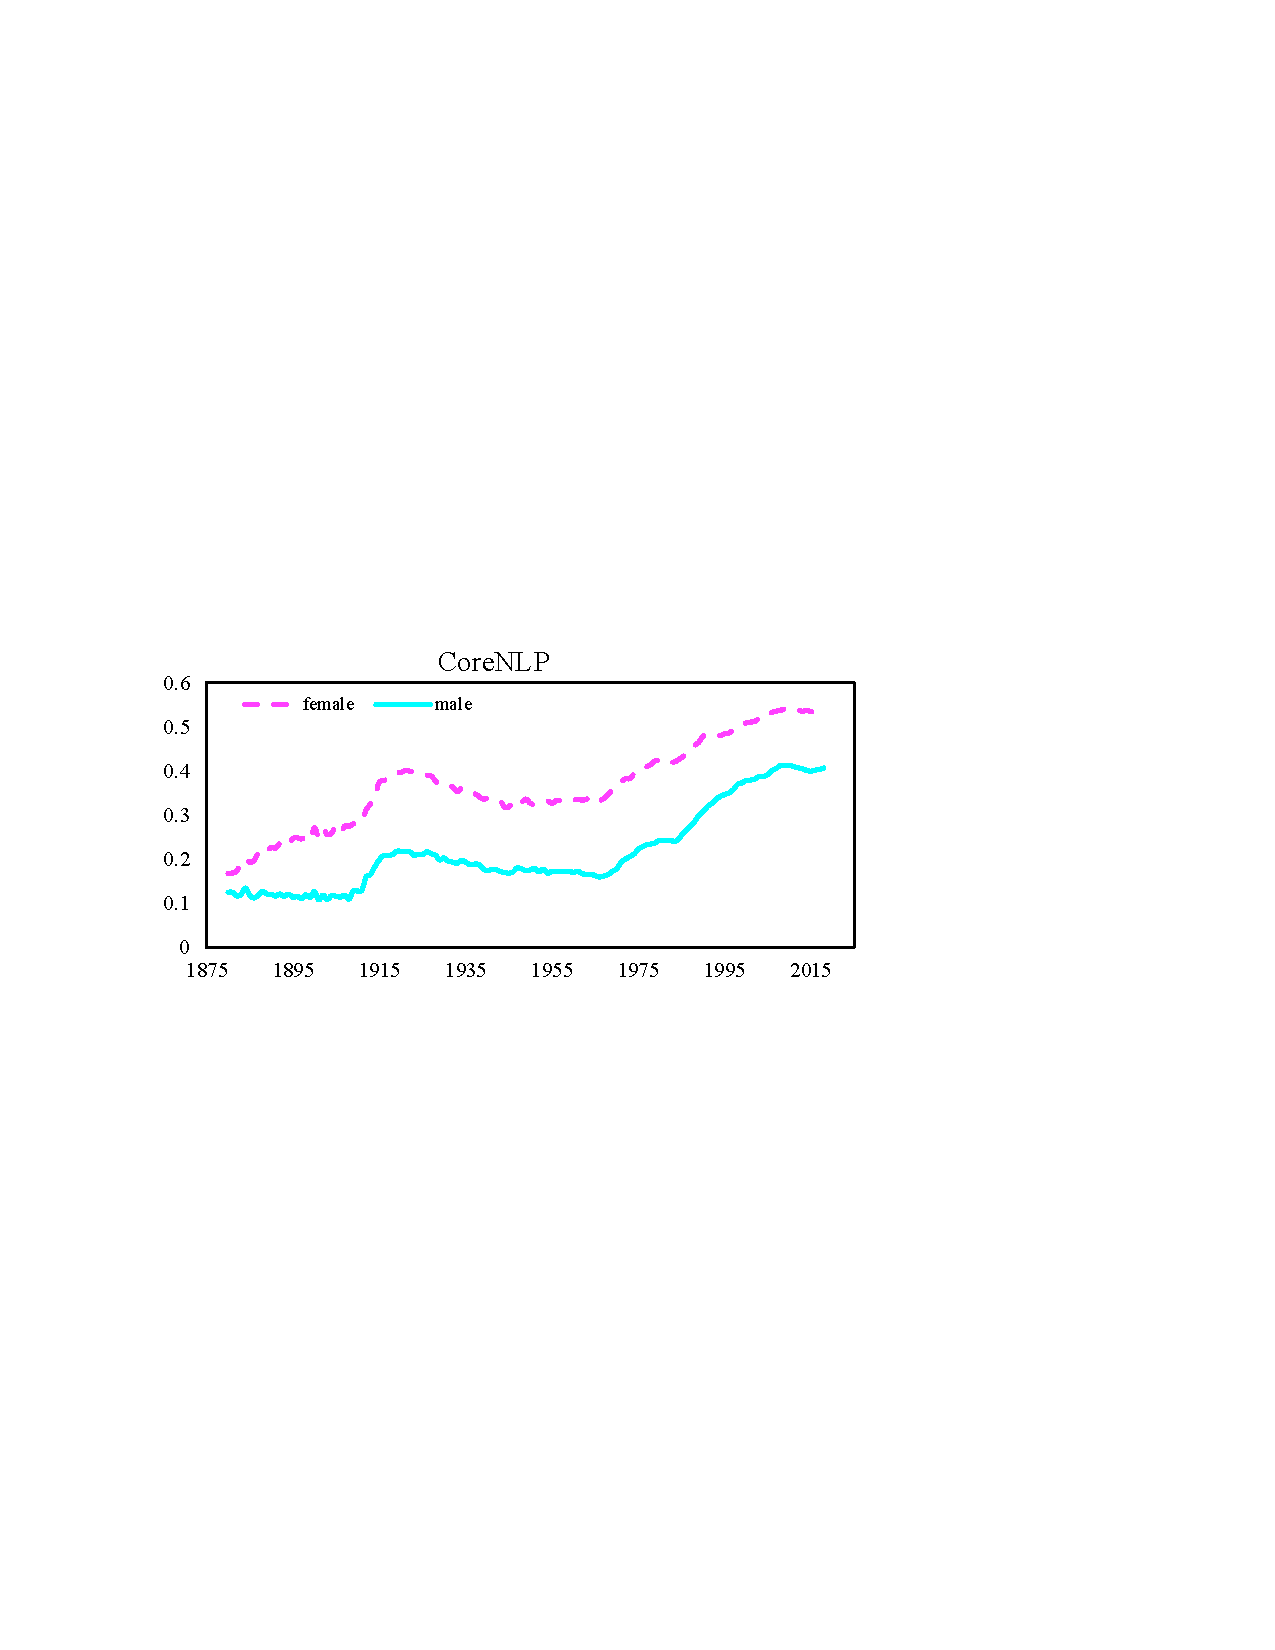
\includegraphics[width=0.196\textwidth,height=0.15\textwidth,trim=0cm 0cm 0cm 0cm,clip=true]{images/unweighted_type3/unweighted_type3_5.pdf}
% \caption{Error Type-3 Unweighted}
% \end{subfigure}
% % \includegraphics[width=\textwidth,height=0.9\textwidth,trim=0cm 0cm 0cm 0cm,clip=true]{unweight_results2.pdf}
% \caption{Results from different models ran over 139 year history of baby names from the census data on different error types for the unweighted case. Female names have higher error rates for all the cases except three marginal cases on error type 3 (not tagged names). The y axis shows the calculated error percentages for each of the error types as described in their coresponding formulas.}
% \label{result2}
% \end{figure*}
